\documentclass[]{book}
\usepackage{amssymb}
\usepackage{amsmath}
\usepackage{times}
\usepackage{listings}
\usepackage{graphicx}
\usepackage{setspace}
\usepackage{tabularx}
\usepackage{longtable}
\pagestyle{plain}
\pagenumbering{arabic}
\oddsidemargin 0.0cm 
\evensidemargin 0.0cm
\topmargin -21pt
\headsep 10pt
\textheight 9.0in 
\textwidth 6.5in
\brokenpenalty=10000
\renewcommand{\baselinestretch}{1.2}

%\renewcommand\citemid{\ } % no comma in optional reference note
\lstset{language=C,frame=TB,basicstyle=\tiny,basicstyle=\ttfamily, %
	xleftmargin=0.25in, xrightmargin=0.25in,captionpos=b, %
	abovecaptionskip=0.5cm, belowcaptionskip=0.5cm, escapeinside={~}{~}}
\renewcommand{\lstlistingname}{Scheme}

\begin{document}

\newcolumntype{A}{p{1.5in}}
\newcolumntype{B}{p{0.75in}}
\newcolumntype{C}{p{1.5in}}
\newcolumntype{D}{p{2in}}

\newcolumntype{E}{p{0.5in}}
\newcolumntype{F}{p{2.25in}}
\newcolumntype{G}{p{3in}}

\newcolumntype{H}{p{0.75in}}
\newcolumntype{I}{p{5in}}


\title{{\sc oopse}-4: An Object-Oriented Parallel Simulation
Engine for Molecular Dynamics}

\author{Teng Lin, Christopher J. Fennell, Charles F. Vardeman II, Xiuquan Sun, \\
Kyle Daily, Yang Zheng, Matthew A. Meineke, and J. Daniel Gezelter\\
Department of Chemistry and Biochemistry\\
University of Notre Dame\\
Notre Dame, Indiana 46556}

\maketitle

\section*{Preface}
{\sc oopse} is a new molecular dynamics simulation program which is
capable of efficiently integrating equations of motion for atom types
with orientational degrees of freedom (e.g. ``sticky'' atoms and point
dipoles).  Transition metals can also be simulated using the embedded
atom method ({\sc eam}) potential included in the code.  Parallel
simulations are carried out using the force-based decomposition
method.  Simulations are specified using a very simple C-based
meta-data language.  A number of advanced integrators are included,
and the basic integrator for orientational dynamics provides
substantial improvements over older quaternion-based schemes.

\tableofcontents
%\listoffigures
%\listoftables
 
\mainmatter

\chapter{\label{sec:intro}Introduction}

There are a number of excellent molecular dynamics packages available
to the chemical physics
community.\cite{Brooks83,MacKerell98,pearlman:1995,Gromacs,Gromacs3,DL_POLY,Tinker,Paradyn,namd,macromodel}
All of these packages are stable, polished programs which solve many
problems of interest.  Most are now capable of performing molecular
dynamics simulations on parallel computers.  Some have source code
which is freely available to the entire scientific community.  Few,
however, are capable of efficiently integrating the equations of
motion for atom types with orientational degrees of freedom
(e.g. point dipoles, and ``sticky'' atoms).  And only one of the
programs referenced can handle transition metal force fields like the
Embedded Atom Method ({\sc eam}).  The direction our research program
has taken us now involves the use of atoms with orientational degrees
of freedom as well as transition metals.  Since these simulation
methods may be of some use to other researchers, we have decided to
release our program (and all related source code) to the scientific
community.

This document communicates the algorithmic details of our program, which
we have been calling the Object-Oriented Parallel Simulation Engine
(i.e. {\sc oopse}).  We have structured this document to first discuss
the underlying concepts in this simulation package
(Sec. \ref{oopseSec:IOfiles}).  The empirical energy functions
implemented are discussed in Sec.~\ref{oopseSec:empiricalEnergy}.
Sec.~\ref{oopseSec:mechanics} describes the various Molecular Dynamics
algorithms {\sc oopse} implements in the integration of Hamilton's
equations of motion.  Program design considerations for parallel
computing are presented in
Sec.~\ref{oopseSec:parallelization}. Concluding remarks are presented
in Sec.~\ref{oopseSec:conclusion}.

\chapter{\label{oopseSec:IOfiles}Concepts \& Files}

A simulation in {\sc oopse} is built using a few fundamental
conceptual building blocks most of which are chemically intuitive.
The basic unit of a simulation is an {\tt atom}.  The parameters
describing an {\tt atom} have been generalized to make it as flexible
as possible; this means that in addition to translational degrees of
freedom, {\tt Atoms} may also have {\it orientational} degrees of freedom.

The fundamental (static) properties of {\tt atoms} are defined by the
{\tt forceField} chosen for the simulation.  The atomic properties
specified by a {\tt forceField} might include (but are not limited to)
charge, $\sigma$ and $\epsilon$ values for Lennard-Jones interactions,
the strength of the dipole moment ($\mu$), the mass, and the moments
of inertia.  Other more complicated properties of atoms might also be
specified by the {\tt forceField}.

{\tt Atoms} can be grouped together in many ways.  A {\tt rigidBody}
contains atoms that exert no forces on one another and which move as a
single rigid unit.  A {\tt cutoffGroup} may contain atoms which
function together as a (rigid {\it or} non-rigid) unit for potential
energy calculations,
\begin{equation}
V_{ab} = s(r_{ab}) \sum_{i \in a} \sum_{j \in b} V_{ij}(r_{ij})
\end{equation}
Here, $a$ and $b$ are two {\tt cutoffGroups} containing multiple atoms
($a = \left\{i\right\}$ and $b = \left\{j\right\}$).  $s(r_{ab})$ is a
generalized switching function which insures that the atoms in the two
{\tt cutoffGroups} are treated identically as the two groups enter or
leave an interaction region.

{\tt Atoms} may also be grouped in more traditional ways into {\tt
bonds}, {\tt bends}, and {\tt torsions}.  These groupings allow the
correct choice of interaction parameters for short-range interactions
to be chosen from the definitions in the {\tt forceField}.

All of these groups of {\tt atoms} are brought together in the {\tt
molecule}, which is the fundamental structure for setting up and {\sc
oopse} simulation.  {\tt Molecules} contain lists of {\tt atoms}
followed by listings of the other atomic groupings ({\tt bonds}, {\tt
bends}, {\tt torsions}, {\tt rigidBodies}, and {\tt cutoffGroups})
which relate the atoms to one another.  Since a {\tt rigidBody} is a
collection of atoms that are propagated in fixed relationships to one
another, {\sc oopse} uses an internal structure called a {\tt
StuntDouble} to store information about those objects that can change
position {\it independently} during a simulation.  That is, an atom
that is part of a rigid body is not itself a StuntDouble.  In this
case, the rigid body is the StuntDouble.  However, an atom that is
free to move independently {\it is} its own StuntDouble.

Simulations often involve heterogeneous collections of molecules.  To
specify a mixture of {\tt molecule} types, {\sc oopse} uses {\tt
components}.  Even simulations containing only one type of molecule
must specify a single {\tt component}.

Starting a simulation requires two types of information: {\it
meta-data}, which describes the types of objects present in the
simulation, and {\it configuration} information, which describes the
initial state of these objects.  An {\sc oopse} file is a single
combined file format that describes both of these kinds of data.  An
{\sc oopse} file contains one {\tt $<$MetaData$>$} block and {\it at least
one} {\tt $<$Snapshot$>$} block.

The language for the {\tt $<$MetaData$>$} block is a C-based syntax that
is parsed at the beginning of the simulation.  Configuration
information is specified for all {\tt integrableObjects} in a {\tt
$<$Snapshot$>$} block.  Both the {\tt $<$MetaData$>$} and {\tt $<$Snapshot$>$}
formats are described in the following sections.

\begin{lstlisting}[float,caption={[The structure of an {\sc oopse} file]
The basic structure of an {\sc oopse} file contains HTML-like tags to
define simulation meta-data and subsequent instantaneous configuration
information. A well-formed {\sc oopse} file must contain one $<$MetaData$>$ 
block and {\it at least one} $<$Snapshot$>$ block.  Each
$<$Snapshot$>$ is further divided into $<$FrameData$>$ and 
$<$StuntDoubles$>$ sections.},
label=sch:oopseFormat]
<OOPSE>
  <MetaData>
      // see section ~\ref{sec:miscConcepts}~ for details on the formatting
      // of information contained inside the <MetaData> tags
  </MetaData>
  <Snapshot>         // An instantaneous configuration
     <FrameData>
                     // FrameData contains information on the time
                     // stamp, the size of the simulation box, and 
                     // the current state of extended system 
                     // ensemble variables.
     </FrameData>
     <StuntDoubles>
                     // StuntDouble information comprises the 
                     // positions, velocities, orientations, and 
                     // angular velocities of anything that is 
                     // capable of independent motion during 
                     // the simulation.
     </StuntDoubles>
  </Snapshot>       
  <Snapshot>         // Multiple <Snapshot> sections can be
  </Snapshot>        // present in a well-formed OOPSE file
  <Snapshot>         // Further information on <Snapshot> blocks
  </Snapshot>        // can be found in section ~\ref{oopseSec:coordFiles}~.
</OOPSE>
\end{lstlisting}


\section{OOPSE Files and $<$MetaData$>$ blocks}

{\sc oopse} uses a HTML-like syntax to separate {\tt $<$MetaData$>$} and
{\tt $<$Snapshot$>$} blocks.  A C-based syntax is used to parse the {\tt
$<$MetaData$>$} blocks at run time.  These blocks allow the user to
completely describe the system they wish to simulate, as well as
tailor {\sc oopse}'s behavior during the simulation.  {\sc oopse}
files are typically denoted with the extension {\tt .md} (which can
stand for Meta-Data or Molecular Dynamics or Molecule Definition
depending on the user's mood). An overview of an {\sc oopse} file is
shown in Scheme~\ref{sch:oopseFormat} and example file is shown in
Scheme~\ref{sch:mdExample}.

\begin{lstlisting}[float,caption={[An example of a complete OOPSE
file] An example showing a complete OOPSE file.},
label={sch:mdExample}] 
<OOPSE>
  <MetaData>
molecule{
  name = "Ar";
  atom[0]{
    type="Ar";
    position( 0.0, 0.0, 0.0 );
  }
}

component{
  type = "Ar";
  nMol = 3;
}

forceField = "LJ";
ensemble = "NVE"; // specify the simulation ensemble
dt = 1.0;         // the time step for integration
runTime = 1e3;    // the total simulation run time
sampleTime = 100; // trajectory file frequency
statusTime = 50;  // statistics file frequency
  </MetaData>
  <Snapshot>
    <FrameData>
        Time: 0
        Hmat: {{ 28.569, 0, 0 }, { 0, 28.569, 0 }, { 0, 0, 28.569 }}
  Thermostat: 0 , 0
    Barostat: {{ 0, 0, 0 }, { 0, 0, 0 }, { 0, 0, 0 }}
    </FrameData>
    <StuntDoubles>
         0      pv   17.5  13.3 12.8  1.181e-03 -1.630e-03 -1.369e-03
         1      pv  -12.8 -14.9 -8.4 -4.440e-04 -2.048e-03  1.130e-03
         2      pv  -10.0 -15.2 -6.5  2.239e-03 -6.310e-03  1.810e-03
    </StuntDoubles>
  </Snapshot>
</OOPSE>
\end{lstlisting}

Within the {\tt $<$MetaData$>$} block it is necessary to provide a
complete description of the molecule before it is actually placed in
the simulation. {\sc oopse}'s meta-data syntax was originally
developed with this goal in mind, and allows for the use of {\it
include files} to specify all atoms in a molecular prototype, as well
as any bonds, bends, or torsions.  Include files allow the user to
describe a molecular prototype once, then simply include it into each
simulation containing that molecule. Returning to the example in
Scheme~\ref{sch:mdExample}, the include file's contents would be
Scheme~\ref{sch:mdIncludeExample}, and the new {\sc oopse} file would
become Scheme~\ref{sch:mdExPrime}.

\begin{lstlisting}[float,caption={An example molecule definition in an
include file.},label={sch:mdIncludeExample}]
molecule{
  name = "Ar";
  atom[0]{
    type="Ar";
    position( 0.0, 0.0, 0.0 );
  }
}
\end{lstlisting}

\begin{lstlisting}[float,caption={Revised OOPSE input file
example.},label={sch:mdExPrime}]
<OOPSE>
  <MetaData>
#include "argon.md"

component{
  type = "Ar";
  nMol = 3;
}

forceField = "LJ";
ensemble = "NVE";
dt = 1.0;
runTime = 1e3;
sampleTime = 100;
statusTime = 50; 
  </MetaData>
  </MetaData>
  <Snapshot$>$
    <FrameData>
        Time: 0
        Hmat: {{ 28.569, 0, 0 }, { 0, 28.569, 0 }, { 0, 0, 28.569 }}
  Thermostat: 0 , 0
    Barostat: {{ 0, 0, 0 }, { 0, 0, 0 }, { 0, 0, 0 }}
    </FrameData>
    <StuntDoubles>
         0      pv   17.5  13.3 12.8  1.181e-03 -1.630e-03 -1.369e-03
         1      pv  -12.8 -14.9 -8.4 -4.440e-04 -2.048e-03  1.130e-03
         2      pv  -10.0 -15.2 -6.5  2.239e-03 -6.310e-03  1.810e-03
    </StuntDoubles>
  </Snapshot>
</OOPSE>
\end{lstlisting}

\section{\label{oopseSec:atomsMolecules}Atoms, Molecules, and other
ways of grouping atoms}

As mentioned above, the fundamental unit for an {\sc oopse} simulation
is the {\tt atom}.  Atoms can be collected into secondary structures
such as {\tt rigidBodies}, {\tt cutoffGroups}, or {\tt molecules}. The
{\tt molecule} is a way for {\sc oopse} to keep track of the atoms in
a simulation in logical manner. Molecular units store the identities
of all the atoms and rigid bodies associated with themselves, and they
are responsible for the evaluation of their own internal interactions
(\emph{i.e.}~bonds, bends, and torsions). Scheme
\ref{sch:mdIncludeExample} shows how one creates a molecule in an
included meta-data file. The positions of the atoms given in the
declaration are relative to the origin of the molecule, and the origin
is used when creating a system containing the molecule.

One of the features that sets {\sc oopse} apart from most of the
current molecular simulation packages is the ability to handle rigid
body dynamics. Rigid bodies are non-spherical particles or collections
of particles (e.g. $\mbox{C}_{60}$) that have a constant internal
potential and move collectively.\cite{Goldstein01} They are not
included in most simulation packages because of the algorithmic
complexity involved in propagating orientational degrees of freedom.
Integrators which propagate orientational motion with an acceptable
level of energy conservation for molecular dynamics are relatively
new inventions.  

Moving a rigid body involves determination of both the force and
torque applied by the surroundings, which directly affect the
translational and rotational motion in turn. In order to accumulate
the total force on a rigid body, the external forces and torques must
first be calculated for all the internal particles. The total force on
the rigid body is simply the sum of these external forces.
Accumulation of the total torque on the rigid body is more complex
than the force because the torque is applied to the center of mass of
the rigid body. The space-fixed torque on rigid body $i$ is
\begin{equation}
\boldsymbol{\tau}_i=
	\sum_{a}\biggl[(\mathbf{r}_{ia}-\mathbf{r}_i)\times \mathbf{f}_{ia} 
	+ \boldsymbol{\tau}_{ia}\biggr],
\label{eq:torqueAccumulate}
\end{equation}
where $\boldsymbol{\tau}_i$ and $\mathbf{r}_i$ are the torque on and
position of the center of mass respectively, while $\mathbf{f}_{ia}$,
$\mathbf{r}_{ia}$, and $\boldsymbol{\tau}_{ia}$ are the force on,
position of, and torque on the component particles of the rigid body.

The summation of the total torque is done in the body fixed axis of
each rigid body. In order to move between the space fixed and body
fixed coordinate axes, parameters describing the orientation must be
maintained for each rigid body. At a minimum, the rotation matrix
($\mathsf{A}$) can be described by the three Euler angles ($\phi,
\theta,$ and $\psi$), where the elements of $\mathsf{A}$ are composed of
trigonometric operations involving $\phi, \theta,$ and
$\psi$.\cite{Goldstein01} In order to avoid numerical instabilities
inherent in using the Euler angles, the four parameter ``quaternion''
scheme is often used. The elements of $\mathsf{A}$ can be expressed as
arithmetic operations involving the four quaternions ($q_w, q_x, q_y,$
and $q_z$).\cite{Allen87} Use of quaternions also leads to
performance enhancements, particularly for very small
systems.\cite{Evans77}

Rather than use one of the previously stated methods, {\sc oopse}
utilizes a relatively new scheme that propagates the entire nine
parameter rotation matrix. Further discussion on this choice can be
found in Sec.~\ref{oopseSec:integrate}. An example definition of a
rigid body can be seen in Scheme
\ref{sch:rigidBody}.

\begin{lstlisting}[float,caption={[Defining rigid bodies]A sample
definition of a molecule containing a rigid body and a cutoff
group},label={sch:rigidBody}] 
molecule{
  name = "TIP3P";
  atom[0]{
    type = "O_TIP3P";
    position( 0.0, 0.0, -0.06556 );
  }
  atom[1]{
    type = "H_TIP3P";
    position( 0.0, 0.75695, 0.52032 );
  }
  atom[2]{
    type = "H_TIP3P";
    position( 0.0, -0.75695, 0.52032 );
  }

  rigidBody[0]{
    members(0, 1, 2);
  }

  cutoffGroup{
    members(0, 1, 2);
  }
}
\end{lstlisting}

\section{\label{sec:miscConcepts}Creating a $<$MetaData$>$ block}

The actual creation of a {\tt $<$MetaData$>$} block requires several key
components. The first part of the file needs to be the declaration of
all of the molecule prototypes used in the simulation. This is
typically done through included prototype files. Only the molecules
actually present in the simulation need to be declared; however, {\sc
oopse} allows for the declaration of more molecules than are
needed. This gives the user the ability to build up a library of
commonly used molecules into a single include file.

Once all prototypes are declared, the ordering of the rest of the
block is less stringent.  The molecular composition of the simulation
is specified with {\tt component} statements. Each different type of
molecule present in the simulation is considered a separate
component (an example is shown in
Sch.~\ref{sch:mdExPrime}).  The component blocks tell {\sc oopse} the
number of molecules that will be in the simulation, and the order in
which the components blocks are declared sets the ordering of the real
atoms in the {\tt $<$Snapshot$>$} block as well as in the output files. The
remainder of the script then sets the various simulation parameters
for the system of interest.

The required set of parameters that must be present in all simulations
is given in Table~\ref{table:reqParams}.  Since the user can use {\sc
oopse} to perform energy minimizations as well as molecular dynamics
simulations, one of the {\tt minimizer} or {\tt ensemble} keywords
must be present.  The {\tt ensemble} keyword is responsible for
selecting the integration method used for the calculation of the
equations of motion. An in depth discussion of the various methods
available in {\sc oopse} can be found in
Sec.~\ref{oopseSec:mechanics}.  The {\tt minimizer} keyword selects
which minimization method to use, and more details on the choices of
minimizer parameters can be found in
Sec.~\ref{oopseSec:minimizer}. The {\tt forceField} statement is
important for the selection of which forces will be used in the course
of the simulation. {\sc oopse} supports several force fields, as
outlined in Sec.~\ref{oopseSec:empiricalEnergy}. The force fields are
interchangeable between simulations, with the only requirement being
that all atoms needed by the simulation are defined within the
selected force field. 

For molecular dynamics simulations, the time step between force
evaluations is set with the {\tt dt} parameter, and {\tt runTime} will
set the time length of the simulation. Note, that {\tt runTime} is an
absolute time, meaning if the simulation is started at t = 10.0~ns
with a {\tt runTime} of 25.0~ns, the simulation will only run for an
additional 15.0~ns.  

For energy minimizations, it is not necessary to specify {\tt dt} or
{\tt runTime}.

To set the initial positions and velocities of all the integrable
objects in the simulation, {\sc oopse} will use the last good {\tt
$<$Snapshot$>$} block that was found in the startup file that it was
called with.  If the {\tt useInitalTime} flag is set to {\tt true},
the time stamp from this snapshot will also set the initial time stamp
for the simulation.  Additional parameters are summarized in
Table~\ref{table:genParams}.

It is important to note the fundamental units in all files which are
read and written by {\sc oopse}.  Energies are in $\mbox{kcal
mol}^{-1}$, distances are in $\mbox{\AA}$, times are in $\mbox{fs}$,
translational velocities are in $\mbox{\AA~fs}^{-1}$, and masses are
in $\mbox{amu}$.  Orientational degrees of freedom are described using
quaternions (unitless, but $q_w^2 + q_x^2 + q_y^2 + q_z^2 = 1$),
body-fixed angular momenta ($\mbox{amu \AA}^{2} \mbox{radians
fs}^{-1}$), and body-fixed moments of inertia ($\mbox{amu \AA}^{2}$). 

\begin{longtable}[c]{ABCD}
\caption{Meta-data Keywords: Required Parameters}
\\
{\bf keyword} & {\bf units} & {\bf use} & {\bf remarks}  \\ \hline
\endhead
\hline
\endfoot
{\tt forceField} & string & Sets the force field. & Possible force
fields are DUFF, WATER, LJ, EAM, SC, and CLAY. \\
{\tt component} & & Defines the molecular components of the system &
Every {\tt $<$MetaData$>$} block must have a component statement. \\
{\tt minimizer} & string & Chooses a minimizer & Possible minimizers
are SD and CG. Either {\tt ensemble} or {\tt minimizer} must be specified. \\
{\tt ensemble} & string & Sets the ensemble. & Possible ensembles are
NVE, NVT, NPTi, NPAT, NPTf, and NPTxyz.  Either {\tt ensemble}
or {\tt minimizer} must be specified. \\
{\tt dt} & fs & Sets the time step. & Selection of {\tt dt} should be
small enough to sample the fastest motion of the simulation. ({\tt
dt} is required for molecular dynamics simulations)\\
{\tt runTime} & fs & Sets the time at which the simulation should
end. & This is an absolute time, and will end the simulation when the
current time meets or exceeds the {\tt runTime}. ({\tt runTime} is
required for molecular dynamics simulations)
\label{table:reqParams}
\end{longtable}

\begin{longtable}[c]{ABCD}
\caption{Meta-data Keywords: Optional Parameters}
\\
{\bf keyword} & {\bf units} & {\bf use} & {\bf remarks}  \\ \hline
\endhead
\hline
\endfoot
{\tt forceFieldVariant} & string & Sets the name of the variant of the
force field.  & {\sc eam} has three variants: {\tt u3}, {\tt u6}, and
{\tt VC}. \\
{\tt forceFieldFileName} & string & Overrides the default force field
file name & Each force field has a default file name, and this
parameter can override the default file name for the chosen force
field. \\
{\tt usePeriodicBoundaryConditions} & & & \\
  & logical & Turns periodic boundary conditions on/off. & Default is true. \\
{\tt orthoBoxTolerance} & double & & decides how orthogonal the periodic
box must be before we can use cheaper box calculations \\
{\tt cutoffRadius} & $\mbox{\AA}$ & Manually sets the cutoff radius &
the default value is set by the {\tt cutoffPolicy} \\ 
{\tt cutoffPolicy} & string & one of mix, max, or
traditional &  the traditional cutoff policy is to set the cutoff
radius for all atoms in the system to the same value (governed by the
largest atom).  mix and max are pair-dependent cutoff
methods. \\
{\tt skinThickness} & \AA & thickness of the skin for the Verlet
neighbor lists & defaults to 1 \AA \\
{\tt switchingRadius} & $\mbox{\AA}$  & Manually sets the inner radius
for the switching function. & Defaults to 85~\% of the {\tt
cutoffRadius}. \\
{\tt switchingFunctionType} & & & \\
 & string & cubic or
fifth\_order\_polynomial & Default is cubic. \\
{\tt useInitialTime} & logical & Sets whether the initial time is
taken from the last $<$Snapshot$>$ in the startup file. & Useful when recovering a simulation from a crashed processor. Default is false. \\
{\tt useInitialExtendedSystemState} & & & \\
  & logical & keep the extended
system variables? & Should the extended
variables (the thermostat and barostat) be kept from the {\tt $<$Snapshot$>$} block? \\
{\tt sampleTime} & fs & Sets the frequency at which the {\tt .dump} file is written. & The default is equal to the {\tt runTime}. \\
{\tt resetTime} & fs & Sets the frequency at which the extended system
variables are reset to zero & The default is to never reset these
variables. \\
{\tt statusTime} & fs & Sets the frequency at which the {\tt .stat} file is written. & The default is equal to the {\tt sampleTime}. \\
{\tt finalConfig} & string & Sets the name of the final output file. & Useful when stringing simulations together. Defaults to the root name of the initial meta-data file but with an {\tt .eor} extension. \\ 
{\tt compressDumpFile} & logical & & should the {\tt .dump} file be
compressed on the fly? \\
{\tt statFileFormat} & string & columns to print in the {\tt .stat}
file where each column is separated by a pipe ($\mid$) symbol. & (The
default is the first eight of these columns in order.)  \\
 & & \multicolumn{2}{p{3.5in}}{Allowed
column names are: {\sc time, total\_energy, potential\_energy, kinetic\_energy,
temperature, pressure, volume, conserved\_quantity,
translational\_kinetic, rotational\_kinetic,  long\_range\_potential,
short\_range\_potential, vanderwaals\_potential,
electrostatic\_potential, bond\_potential, bend\_potential,
dihedral\_potential, improper\_potential, vraw, vharm,
pressure\_tensor\_x, pressure\_tensor\_y, pressure\_tensor\_z}} \\
{\tt printPressureTensor} & logical & sets whether OOPSE will print
out the pressure tensor & can be useful for calculations of the bulk
modulus \\
{\tt electrostaticSummationMethod} & & & \\
 & string & shifted\_force,
shifted\_potential, shifted\_force, or reaction\_field &
default is shifted\_force. \\
{\tt electrostaticScreeningMethod} & & & \\
 & string & undamped or damped & default is damped \\
{\tt dielectric} & unitless & Sets the dielectric constant for
reaction field. & If {\tt electrostaticSummationMethod} is set to {\tt
reaction\_field}, then {\tt dielectric} must be set. \\
{\tt dampingAlpha} & $\mbox{\AA}^{-1}$ & governs strength of
electrostatic damping & defaults to 0.2 $\mbox{\AA}^{-1}$. \\
{\tt tempSet} & logical & resample velocities from a Maxwell-Boltzmann
distribution set to {\tt targetTemp} & default is false. \\
{\tt thermalTime} & fs & how often to perform a {\tt tempSet} &
default is never \\
{\tt targetTemp} & K & sets the target temperature & no default value \\
{\tt tauThermostat} & fs & time constant for Nos\'{e}-Hoover
thermostat & times from 1000-10,000 fs are reasonable \\
{\tt targetPressure} & atm & sets the target pressure & no default value\\
{\tt surfaceTension} &  & sets the target surface tension in the x-y
plane & no default value \\
{\tt tauBarostat} & fs & time constant for the
Nos\'{e}-Hoover-Andersen barostat & times from 10,000 to 100,000 fs
are reasonable \\
{\tt seed } & integer & Sets the seed value for the random number generator. & The seed needs to be at least 9 digits long. The default is to take the seed from the CPU clock. \\
\label{table:genParams}
\end{longtable}


\section{\label{oopseSec:coordFiles}$<$Snapshot$>$ Blocks}

The standard format for storage of a system's coordinates is the {\tt
$<$Snapshot$>$} block , the exact details of which can be seen in
Scheme~\ref{sch:dumpFormat}. As all bonding and molecular information
is stored in the {\tt $<$MetaData$>$} blocks, the {\tt $<$Snapshot$>$} blocks
contain only the coordinates of the objects which move independently
during the simulation.  It is important to note that {\it not all
atoms} are capable of independent motion.  Atoms which are part of
rigid bodies are not ``integrable objects'' in the equations of
motion; the rigid bodies themselves are the integrable objects.
Therefore, the coordinate file contains coordinates of all the {\tt
integrableObjects} in the system.  For systems without rigid bodies,
this is simply the coordinates of all the atoms.

It is important to note that although the simulation propagates the
complete rotation matrix, directional entities are written out using
quaternions to save space in the output files.

\begin{lstlisting}[float,caption={[The format of the {\tt $<$Snapshot$>$} block]
An example of the format of the {\tt $<$Snapshot$>$} block.  There is an
initial sub-block called {\tt $<$FrameData$>$} which contains the time
stamp, the three column vectors of $\mathsf{H}$, and optional extra
information for the extended sytem ensembles.  The lines in the {\tt
$<$StuntDoubles$>$} sub-block provide information about the instantaneous
configuration of each integrable object.  For each integrable object,
the global index is followed by a short string describing what
additional information is present on the line.  Atoms with only
position and velocity information use the ``pv'' string which must
then be followed by the position and velocity vectors for that atom.
Directional atoms and Rigid Bodies typically use the ``pvqj'' string
which is followed by position, velocity, quaternions, and
lastly, body fixed angular momentum for that integrable object.},
label=sch:dumpFormat]
  <Snapshot>
    <FrameData>
        Time: 0
        Hmat: {{ Hxx, Hyx, Hzx }, { Hxy, Hyy, Hzy }, { Hxz, Hyz, Hzz }}
  Thermostat: 0 , 0
    Barostat: {{ 0, 0, 0 }, { 0, 0, 0 }, { 0, 0, 0 }}
    </FrameData>
    <StuntDoubles>
         0      pv          x y z vx vy vz
         1      pv          x y z vx vy vz
         2      pvqj        x y z vx vy vz  qw qx qy qz jx jy jz
         3      pvqj        x y z vx vy vz  qw qx qy qz jx jy jz
    </StuntDoubles>
  </Snapshot>
\end{lstlisting}

There are three {\sc oopse} files that are written using the combined
format.  They are: the initial startup file (\texttt{.md}), the
simulation trajectory file (\texttt{.dump}), and the final coordinates
or ``end-of-run'' for the simulation (\texttt{.eor}). The initial
startup file is necessary for {\sc oopse} to start the simulation with
the proper coordinates, and this file must be generated by the user
before the simulation run. The trajectory (or ``dump'') file is
updated during simulation and is used to store snapshots of the
coordinates at regular intervals. The first frame is a duplication of
the initial configuration (the last good {\tt $<$Snapshot$>$} in the
startup file), and each subsequent frame is appended to the dump file
at an interval specified in the meta-data file with the
\texttt{sampleTime} flag. The final coordinate file is the
``end-of-run'' file.  The \texttt{.eor} file stores the final
configuration of the system for a given simulation. The file is
updated at the same time as the \texttt{.dump} file, but it only
contains the most recent frame. In this way, an \texttt{.eor} file may
be used to initialize a second simulation should it be necessary to
recover from a crash or power outage. The coordinate files generated
by {\sc oopse} (both \texttt{.dump} and \texttt{.eor}) all contain the
same {\tt $<$MetaData$>$} block as the startup file, so they may be
used to start up a new simulation if desired.

\section{\label{oopseSec:initCoords}Generation of Initial Coordinates}

As was stated in Sec.~\ref{oopseSec:coordFiles}, a meaningful {\tt
$<$Snapshot$>$} block is necessary for specifying for the starting
coordinates for a simulation.  Since each simulation is different,
system creation is left to the end user; however, we have included a
few sample programs which make some specialized structures.  The {\tt
$<$Snapshot$>$} block must index the integrable objects in the correct
order.  The ordering of the integrable objects relies on the ordering
of molecules within the {\tt $<$MetaData$>$} block. {\sc oopse}
expects the order to comply with the following guidelines:
\begin{enumerate}
\item All of the molecules of the first declared component are given
before proceeding to the molecules of the second component, and so on
for all subsequently declared components.
\item The ordering of the atoms for each molecule follows the order
declared in the molecule's declaration within the model file.
\item Only atoms which are not members of a {\tt rigidBody} are
included.
\item Rigid Body coordinates for a molecule are listed immediately
after the the other atoms in a molecule.  Some molecules may be
entirely rigid, in which case, only the rigid body coordinates are
given.
\end{enumerate}
An example is given in the {\sc oopse} file in Scheme~\ref{sch:initEx1}.

\begin{lstlisting}[float,caption={Example declaration of the
$\text{I}_2$ molecule and the HCl molecule in $<$MetaData$>$ and
$<$Snapshot$>$ blocks.  Note that even though $\text{I}_2$ is
declared before HCl, the $<$Snapshot$>$ block follows the order {\it in
which the components were included}.}, label=sch:initEx1] 
<OOPSE>
  <MetaData>
molecule{
  name = "I2";
  atom[0]{
    type = "I";
  }
  atom[1]{
    type = "I";
  }
  bond{
    members( 0, 1);
  }
}
molecule{
  name = "HCl"
  atom[0]{
    type = "H";
  }
  atom[1]{
    type = "Cl";
  }
  bond{
    members( 0, 1);
  }
}
component{
  type = "HCl";
  nMol = 4;
}
component{
  type = "I2";
  nMol = 1;
}
  </MetaData>
  <Snapshot>
    <FrameData>
        Time: 0
        Hmat: {{ 10.0, 0.0, 0.0 }, { 0.0, 10.0, 0.0 }, { 0.0, 0.0, 10.0 }}
    </FrameData>
    <StuntDoubles>
         0      pv          x y z vx vy vz // H from first HCl molecule 
         1      pv          x y z vx vy vz // Cl from first HCl molecule
         2      pv          x y z vx vy vz // H from second HCl molecule 
         3      pv          x y z vx vy vz // Cl from second HCl molecule
         4      pv          x y z vx vy vz // H from third HCl molecule 
         5      pv          x y z vx vy vz // Cl from third HCl molecule
         6      pv          x y z vx vy vz // H from fourth HCl molecule 
         7      pv          x y z vx vy vz // Cl from fourth HCl molecule
         8      pv          x y z vx vy vz // First I from I2 molecule
         9      pv          x y z vx vy vz // Second I from I2 molecule
    </StuntDoubles>
  </Snapshot>
</OOPSE>
\end{lstlisting}

\section{The Statistics File}

The last output file generated by {\sc oopse} is the statistics
file. This file records such statistical quantities as the
instantaneous temperature (in $K$), volume (in $\mbox{\AA}^{3}$),
pressure (in $\mbox{atm}$), etc. It is written out with the frequency
specified in the meta-data file with the
\texttt{statusTime} keyword. The file allows the user to observe the
system variables as a function of simulation time while the simulation
is in progress. One useful function the statistics file serves is to
monitor the conserved quantity of a given simulation ensemble,
allowing the user to gauge the stability of the integrator. The
statistics file is denoted with the \texttt{.stat} file extension.

\chapter{\label{oopseSec:empiricalEnergy}The Empirical Energy
Functions}

Like many simulation packages, {\sc oopse} splits the potential energy
into the short-ranged (bonded) portion and a long-range (non-bonded)
potential,
\begin{equation}
V = V_{\mathrm{short-range}} + V_{\mathrm{long-range}}.
\end{equation}
The short-ranged portion includes the explicit bonds, bends, and
torsions which have been defined in the meta-data file for the
molecules which are present in the simulation.  The functional forms and
parameters for these interactions are defined by the force field which
is chosen.

Calculating the long-range (non-bonded) potential involves a sum over
all pairs of atoms (except for those atoms which are involved in a
bond, bend, or torsion with each other).  If done poorly, calculating
the the long-range interactions for $N$ atoms would involve $N(N-1)/2$
evaluations of atomic distances.  To reduce the number of distance
evaluations between pairs of atoms, {\sc oopse} uses a switched cutoff
with Verlet neighbor lists.\cite{Allen87} It is well known that
neutral groups which contain charges will exhibit pathological forces
unless the cutoff is applied to the neutral groups evenly instead of
to the individual atoms.\cite{leach01:mm} {\sc oopse} allows users to
specify cutoff groups which may contain an arbitrary number of atoms
in the molecule.  Atoms in a cutoff group are treated as a single unit
for the evaluation of the switching function:
\begin{equation}
V_{\mathrm{long-range}} = \sum_{a} \sum_{b>a} s(r_{ab}) \sum_{i \in a} \sum_{j \in b} V_{ij}(r_{ij}),
\end{equation}
where $r_{ab}$ is the distance between the centers of mass of the two
cutoff groups ($a$ and $b$).

The sums over $a$ and $b$ are over the cutoff groups that are present
in the simulation.  Atoms which are not explicitly defined as members
of a {\tt cutoffGroup} are treated as a group consisting of only one
atom.  The switching function, $s(r)$ is the standard cubic switching
function,
\begin{equation}
S(r) = 
	\begin{cases}
	1 & \text{if $r \le r_{\text{sw}}$},\\
	\frac{(r_{\text{cut}} + 2r - 3r_{\text{sw}})(r_{\text{cut}} - r)^2}
	{(r_{\text{cut}} - r_{\text{sw}})^3} 
	& \text{if $r_{\text{sw}} < r \le r_{\text{cut}}$}, \\
	0 & \text{if $r > r_{\text{cut}}$.}
	\end{cases}
\label{eq:dipoleSwitching}
\end{equation}
Here, $r_{\text{sw}}$ is the {\tt switchingRadius}, or the distance
beyond which interactions are reduced, and $r_{\text{cut}}$ is the
{\tt cutoffRadius}, or the distance at which interactions are
truncated.

Users of {\sc oopse} do not need to specify the {\tt cutoffRadius} or
{\tt switchingRadius}.  In simulations containing only Lennard-Jones
atoms, the cutoff radius has a default value of $2.5\sigma_{ii}$,
where $\sigma_{ii}$ is the largest Lennard-Jones length parameter
present in the simulation.  In simulations containing charged or
dipolar atoms, the default cutoff radius is $15 \mbox{\AA}$.  

The {\tt switchingRadius} is set to a default value of 95\% of the
{\tt cutoffRadius}.  In the special case of a simulation containing
{\it only} Lennard-Jones atoms, the default switching radius takes the
same value as the cutoff radius, and {\sc oopse} will use a shifted
potential to remove discontinuities in the potential at the cutoff.
Both radii may be specified in the meta-data file.

Force fields can be added to {\sc oopse}, although it comes with a few
simple examples (Lennard-Jones, {\sc duff}, {\sc water}, and {\sc
eam}) which are explained in the following sections.

\section{\label{sec:LJPot}The Lennard Jones Force Field}

The most basic force field implemented in {\sc oopse} is the
Lennard-Jones force field, which mimics the van der Waals interaction
at long distances and uses an empirical repulsion at short
distances. The Lennard-Jones potential is given by:
\begin{equation}
V_{\text{LJ}}(r_{ij}) = 
	4\epsilon_{ij} \biggl[
	\biggl(\frac{\sigma_{ij}}{r_{ij}}\biggr)^{12}
	- \biggl(\frac{\sigma_{ij}}{r_{ij}}\biggr)^{6}
	\biggr],
\label{eq:lennardJonesPot}
\end{equation}
where $r_{ij}$ is the distance between particles $i$ and $j$,
$\sigma_{ij}$ scales the length of the interaction, and
$\epsilon_{ij}$ scales the well depth of the potential. Scheme
\ref{sch:LJFF} gives an example meta-data file that
sets up a system of 108 Ar particles to be simulated using the
Lennard-Jones force field.

\begin{lstlisting}[float,caption={[Invocation of the Lennard-Jones
force field] A sample startup file for a small Lennard-Jones
simulation.},label={sch:LJFF}]
<OOPSE>
  <MetaData>
#include "argon.md" 

component{
  type = "Ar";
  nMol = 108;
}

forceField = "LJ";
  </MetaData>
  <Snapshot>     // not shown in this scheme
  </Snapshot>
</OOPSE>
\end{lstlisting}

Interactions between dissimilar particles requires the generation of
cross term parameters for $\sigma$ and $\epsilon$. These parameters
are determined using the Lorentz-Berthelot mixing
rules:\cite{Allen87}
\begin{equation}
\sigma_{ij} = \frac{1}{2}[\sigma_{ii} + \sigma_{jj}],
\label{eq:sigmaMix}
\end{equation}
and
\begin{equation}
\epsilon_{ij} = \sqrt{\epsilon_{ii} \epsilon_{jj}}.
\label{eq:epsilonMix}
\end{equation}

\section{\label{oopseSec:DUFF}Dipolar Unified-Atom Force Field}

The dipolar unified-atom force field ({\sc duff}) was developed to
simulate lipid bilayers. These types of simulations require a model
capable of forming bilayers, while still being sufficiently
computationally efficient to allow large systems ($\sim$100's of
phospholipids, $\sim$1000's of waters) to be simulated for long times
($\sim$10's of nanoseconds). With this goal in mind, {\sc duff} has no
point charges. Charge-neutral distributions are replaced with dipoles,
while most atoms and groups of atoms are reduced to Lennard-Jones
interaction sites. This simplification reduces the length scale of
long range interactions from $\frac{1}{r}$ to $\frac{1}{r^3}$,
removing the need for the computationally expensive Ewald
sum. Instead, Verlet neighbor-lists and cutoff radii are used for the
dipolar interactions, and, if desired, a reaction field may be added
to mimic longer range interactions.

As an example, lipid head-groups in {\sc duff} are represented as
point dipole interaction sites.  Placing a dipole at the head group's
center of mass mimics the charge separation found in common
phospholipid head groups such as phosphatidylcholine.\cite{Cevc87}
Additionally, a large Lennard-Jones site is located at the
pseudoatom's center of mass. The model is illustrated by the red atom
in Fig.~\ref{oopseFig:lipidModel}. The water model we use to
complement the dipoles of the lipids is a
reparameterization\cite{fennell04} of the soft sticky dipole (SSD)
model of Ichiye
\emph{et al.}\cite{liu96:new_model}

\begin{figure}
\centering
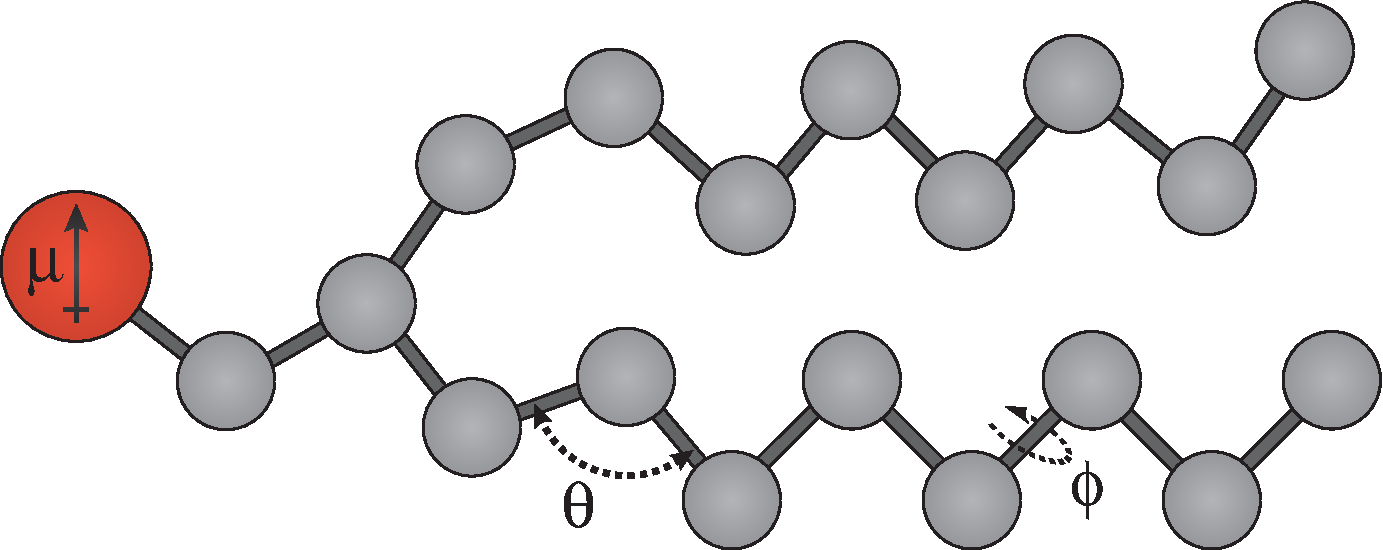
\includegraphics[width=\linewidth]{lipidModel.pdf}
\caption[A representation of a lipid model in {\sc duff}]{A
representation of the lipid model. $\phi$ is the torsion angle,
$\theta$ is the bend angle, and $\mu$ is the dipole moment of the head
group.}
\label{oopseFig:lipidModel}
\end{figure}

A set of scalable parameters has been used to model the alkyl groups
with Lennard-Jones sites. For this, parameters from the TraPPE force
field of Siepmann \emph{et al.}\cite{Siepmann1998} have been
utilized. TraPPE is a unified-atom representation of n-alkanes which
is parametrized against phase equilibria using Gibbs ensemble Monte
Carlo simulation techniques.\cite{Siepmann1998} One of the advantages
of TraPPE is that it generalizes the types of atoms in an alkyl chain
to keep the number of pseudoatoms to a minimum; thus, the parameters
for a unified atom such as $\text{CH}_2$ do not change depending on
what species are bonded to it.

As is required by TraPPE, {\sc duff} also constrains all bonds to be
of fixed length. Typically, bond vibrations are the fastest motions in
a molecular dynamic simulation.  With these vibrations present, small
time steps between force evaluations must be used to ensure adequate
energy conservation in the bond degrees of freedom. By constraining
the bond lengths, larger time steps may be used when integrating the
equations of motion. A simulation using {\sc duff} is illustrated in
Scheme \ref{sch:DUFF}.

\begin{lstlisting}[float,caption={[Invocation of {\sc duff}]A portion
of a startup file showing a simulation utilizing {\sc
duff}},label={sch:DUFF}]  
<OOPSE>
  <MetaData>
#include "water.md"
#include "lipid.md"

component{
  type = "simpleLipid_16";
  nMol = 60;
}

component{
  type = "SSD_water";
  nMol = 1936;
}

forceField = "DUFF";
  </MetaData>
  <Snapshot>     // not shown in this scheme
  </Snapshot>
</OOPSE
\end{lstlisting}

\subsection{\label{oopseSec:energyFunctions}{\sc duff} Energy Functions}

The total potential energy function in {\sc duff} is
\begin{equation}
V = \sum^{N}_{I=1} V^{I}_{\text{Internal}}
	+ \sum^{N-1}_{I=1} \sum_{J>I} V^{IJ}_{\text{Cross}},
\label{eq:totalPotential}
\end{equation}
where $V^{I}_{\text{Internal}}$ is the internal potential of molecule $I$:
\begin{equation}
 V^{I}_{\text{Internal}} = 
	\sum_{\theta_{ijk} \in I} V_{\text{bend}}(\theta_{ijk})
	+ \sum_{\phi_{ijkl} \in I} V_{\text{torsion}}(\phi_{ijkl})
	+ \sum_{i \in I} \sum_{(j>i+4) \in I} 
	\biggl[ V_{\text{LJ}}(r_{ij}) +  V_{\text{dipole}}
	(\mathbf{r}_{ij},\boldsymbol{\Omega}_{i},\boldsymbol{\Omega}_{j})
	\biggr].
\label{eq:internalPotential}
\end{equation}
Here $V_{\text{bend}}$ is the bend potential for all 1, 3 bonded pairs
within the molecule $I$, and $V_{\text{torsion}}$ is the torsion
potential for all 1, 4 bonded pairs.  The pairwise portions of the
non-bonded interactions are excluded for atom pairs that are involved
in the smae bond, bend, or torsion. All other atom pairs within a
molecule are subject to the LJ pair potential.

The bend potential of a molecule is represented by the following function:
\begin{equation}
V_{\text{bend}}(\theta_{ijk}) = k_{\theta}( \theta_{ijk} - \theta_0
)^2, \label{eq:bendPot}
\end{equation}
where $\theta_{ijk}$ is the angle defined by atoms $i$, $j$, and $k$
(see Fig.~\ref{oopseFig:lipidModel}), $\theta_0$ is the equilibrium
bond angle, and $k_{\theta}$ is the force constant which determines the
strength of the harmonic bend. The parameters for $k_{\theta}$ and
$\theta_0$ are borrowed from those in TraPPE.\cite{Siepmann1998}

The torsion potential and parameters are also borrowed from TraPPE. It is
of the form:
\begin{equation}
V_{\text{torsion}}(\phi) = c_1[1 + \cos \phi] 
	+ c_2[1 + \cos(2\phi)] 
 	+ c_3[1 + \cos(3\phi)],
\label{eq:origTorsionPot}
\end{equation}
where:
\begin{equation}
\cos\phi = (\hat{\mathbf{r}}_{ij} \times \hat{\mathbf{r}}_{jk}) \cdot
	(\hat{\mathbf{r}}_{jk} \times \hat{\mathbf{r}}_{kl}).
\label{eq:torsPhi}
\end{equation}
Here, $\hat{\mathbf{r}}_{\alpha\beta}$ are the set of unit bond
vectors between atoms $i$, $j$, $k$, and $l$. For computational
efficiency, the torsion potential has been recast after the method of
{\sc charmm},\cite{Brooks83} in which the angle series is converted to
a power series of the form:
\begin{equation}
V_{\text{torsion}}(\phi) =  
	k_3 \cos^3 \phi + k_2 \cos^2 \phi + k_1 \cos \phi + k_0,
\label{eq:torsionPot}
\end{equation}
where:
\begin{align*}
k_0 &= c_1 + c_3, \\
k_1 &= c_1 - 3c_3, \\
k_2 &= 2 c_2, \\
k_3 &= 4c_3.
\end{align*}
By recasting the potential as a power series, repeated trigonometric
evaluations are avoided during the calculation of the potential
energy.


The cross potential between molecules $I$ and $J$,
$V^{IJ}_{\text{Cross}}$, is as follows:
\begin{equation}
V^{IJ}_{\text{Cross}} = 
	\sum_{i \in I} \sum_{j \in J}
	\biggl[ V_{\text{LJ}}(r_{ij}) +  V_{\text{dipole}}
	(\mathbf{r}_{ij},\boldsymbol{\Omega}_{i},\boldsymbol{\Omega}_{j})
	+ V_{\text{sticky}}
	(\mathbf{r}_{ij},\boldsymbol{\Omega}_{i},\boldsymbol{\Omega}_{j})
	\biggr],
\label{eq:crossPotentail}
\end{equation}
where $V_{\text{LJ}}$ is the Lennard Jones potential,
$V_{\text{dipole}}$ is the dipole dipole potential, and
$V_{\text{sticky}}$ is the sticky potential defined by the SSD model
(Sec.~\ref{oopseSec:SSD}). Note that not all atom types include all
interactions.

The dipole-dipole potential has the following form:
\begin{equation}
V_{\text{dipole}}(\mathbf{r}_{ij},\boldsymbol{\Omega}_{i},
	\boldsymbol{\Omega}_{j}) = \frac{|\mu_i||\mu_j|}{4\pi\epsilon_{0}r_{ij}^{3}} \biggl[
	\boldsymbol{\hat{u}}_{i} \cdot \boldsymbol{\hat{u}}_{j}
	-
	3(\boldsymbol{\hat{u}}_i \cdot \hat{\mathbf{r}}_{ij}) %
		(\boldsymbol{\hat{u}}_j \cdot \hat{\mathbf{r}}_{ij}) \biggr].
\label{eq:dipolePot}
\end{equation}
Here $\mathbf{r}_{ij}$ is the vector starting at atom $i$ pointing
towards $j$, and $\boldsymbol{\Omega}_i$ and $\boldsymbol{\Omega}_j$
are the orientational degrees of freedom for atoms $i$ and $j$
respectively. The magnitude of the dipole moment of atom $i$ is
$|\mu_i|$, $\boldsymbol{\hat{u}}_i$ is the standard unit orientation
vector of $\boldsymbol{\Omega}_i$, and $\boldsymbol{\hat{r}}_{ij}$ is
the unit vector pointing along $\mathbf{r}_{ij}$
($\boldsymbol{\hat{r}}_{ij}=\mathbf{r}_{ij}/|\mathbf{r}_{ij}|$).

\subsection{\label{oopseSec:SSD}The {\sc duff} Water Models: SSD/E
and SSD/RF} 

In the interest of computational efficiency, the default solvent used
by {\sc oopse} is the extended Soft Sticky Dipole (SSD/E) water
model.\cite{fennell04} The original SSD was developed by Ichiye
\emph{et al.}\cite{liu96:new_model} as a modified form of the hard-sphere 
water model proposed by Bratko, Blum, and
Luzar.\cite{Bratko85,Bratko95} It consists of a single point dipole
with a Lennard-Jones core and a sticky potential that directs the
particles to assume the proper hydrogen bond orientation in the first
solvation shell. Thus, the interaction between two SSD water molecules
\emph{i} and \emph{j} is given by the potential
\begin{equation}
V_{ij} = 
	V_{ij}^{LJ} (r_{ij})\ + V_{ij}^{dp}
	(\mathbf{r}_{ij},\boldsymbol{\Omega}_i,\boldsymbol{\Omega}_j)\ +
	V_{ij}^{sp}
	(\mathbf{r}_{ij},\boldsymbol{\Omega}_i,\boldsymbol{\Omega}_j),
\label{eq:ssdPot}
\end{equation}
where the $\mathbf{r}_{ij}$ is the position vector between molecules
\emph{i} and \emph{j} with magnitude equal to the distance $r_{ij}$, and
$\boldsymbol{\Omega}_i$ and $\boldsymbol{\Omega}_j$ represent the
orientations of the respective molecules. The Lennard-Jones and dipole
parts of the potential are given by equations \ref{eq:lennardJonesPot}
and \ref{eq:dipolePot} respectively. The sticky part is described by
the following,
\begin{equation}
u_{ij}^{sp}(\mathbf{r}_{ij},\boldsymbol{\Omega}_i,\boldsymbol{\Omega}_j)=
	\frac{\nu_0}{2}[s(r_{ij})w(\mathbf{r}_{ij},
	\boldsymbol{\Omega}_i,\boldsymbol{\Omega}_j) +
	s^\prime(r_{ij})w^\prime(\mathbf{r}_{ij},
	\boldsymbol{\Omega}_i,\boldsymbol{\Omega}_j)]\ ,
\label{eq:stickyPot}
\end{equation}
where $\nu_0$ is a strength parameter for the sticky potential, and
$s$ and $s^\prime$ are cubic switching functions which turn off the
sticky interaction beyond the first solvation shell. The $w$ function
can be thought of as an attractive potential with tetrahedral
geometry:
\begin{equation}
w({\bf r}_{ij},{\bf \Omega}_i,{\bf \Omega}_j)=
	\sin\theta_{ij}\sin2\theta_{ij}\cos2\phi_{ij},
\label{eq:stickyW}
\end{equation}
while the $w^\prime$ function counters the normal aligned and
anti-aligned structures favored by point dipoles:
\begin{equation}
w^\prime({\bf r}_{ij},{\bf \Omega}_i,{\bf \Omega}_j)=
	(\cos\theta_{ij}-0.6)^2(\cos\theta_{ij}+0.8)^2-w^0,
\label{eq:stickyWprime}
\end{equation}
It should be noted that $w$ is proportional to the sum of the $Y_3^2$
and $Y_3^{-2}$ spherical harmonics (a linear combination which
enhances the tetrahedral geometry for hydrogen bonded structures),
while $w^\prime$ is a purely empirical function.  A more detailed
description of the functional parts and variables in this potential
can be found in the original SSD
articles.\cite{liu96:new_model,liu96:monte_carlo,chandra99:ssd_md,Ichiye03}

\begin{figure}
\centering
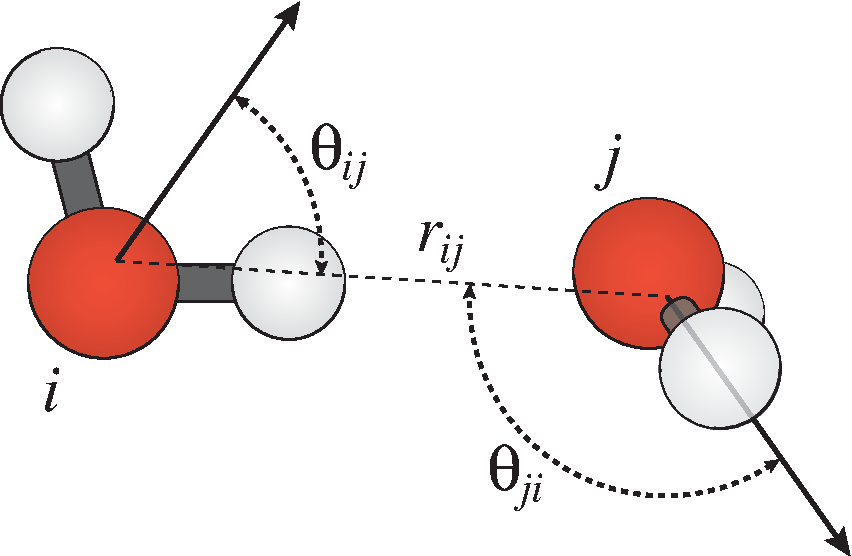
\includegraphics[width=\linewidth]{waterAngle.pdf}
\caption[Coordinate definition for the SSD/E water model]{Coordinates
for the interaction between two SSD/E water molecules.  $\theta_{ij}$
is the angle that $r_{ij}$ makes with the $\hat{z}$ vector in the
body-fixed frame for molecule $i$.  The $\hat{z}$ vector bisects the
HOH angle in each water molecule. } 
\label{oopseFig:ssd}
\end{figure}


Since SSD/E is a single-point {\it dipolar} model, the force
calculations are simplified significantly relative to the standard
{\it charged} multi-point models. In the original Monte Carlo
simulations using this model, Ichiye {\it et al.} reported that using
SSD decreased computer time by a factor of 6-7 compared to other
models.\cite{liu96:new_model} What is most impressive is that these
savings did not come at the expense of accurate depiction of the
liquid state properties.  Indeed, SSD/E maintains reasonable agreement
with the Head-Gordon diffraction data for the structural features of
liquid water.\cite{hura00,liu96:new_model} Additionally, the dynamical
properties exhibited by SSD/E agree with experiment better than those
of more computationally expensive models (like TIP3P and
SPC/E).\cite{chandra99:ssd_md} The combination of speed and accurate
depiction of solvent properties makes SSD/E a very attractive model
for the simulation of large scale biochemical simulations.

Recent constant pressure simulations revealed issues in the original
SSD model that led to lower than expected densities at all target
pressures.\cite{Ichiye03,fennell04} The default model in {\sc oopse}
is therefore SSD/E, a density corrected derivative of SSD that
exhibits improved liquid structure and transport behavior. If the use
of a reaction field long-range interaction correction is desired, it
is recommended that the parameters be modified to those of the SSD/RF
model (an SSD variant parameterized for reaction field). These solvent
parameters are listed and can be easily modified in the {\sc duff}
force field file ({\tt DUFF.frc}).  A table of the parameter values
and the drawbacks and benefits of the different density corrected SSD
models can be found in reference~\cite{fennell04}. 

\section{\label{oopseSec:WATER}The {\sc water} Force Field}

In addition to the {\sc duff} force field's solvent description, a
separate {\sc water} force field has been included for simulating most
of the common rigid-body water models. This force field includes the
simple and point-dipolar models (SSD, SSD1, SSD/E, SSD/RF, and DPD
water), as well as the common charge-based models (SPC, SPC/E, TIP3P,
TIP4P, and
TIP5P).\cite{liu96:new_model,Ichiye03,fennell04,Marrink01,Berendsen81,Berendsen87,Jorgensen83,Mahoney00}
In order to handle these models, charge-charge interactions were
included in the force-loop:
\begin{equation}
V_{\text{charge}}(r_{ij}) = \sum_{ij}\frac{q_iq_je^2}{r_{ij}}, 
\end{equation}
where $q$ represents the charge on particle $i$ or $j$, and $e$ is the
charge of an electron in Coulombs. The charge-charge interaction
support is rudimentary in the current version of {\sc oopse}.  As with
the other pair interactions, charges can be simulated with a pure
cutoff or a reaction field.  The various methods for performing the
Ewald summation have not yet been included.  The {\sc water} force
field can be easily expanded through modification of the {\sc water}
force field file ({\tt WATER.frc}). By adding atom types and inserting
the appropriate parameters, it is possible to extend the force field
to handle rigid molecules other than water.

\section{\label{oopseSec:eam}Embedded Atom Method}

{\sc oopse} implements a potential that describes bonding in
transition metal
systems.~\cite{Finnis84,Ercolessi88,Chen90,Qi99,Ercolessi02} This
potential has an attractive interaction which models ``Embedding'' a
positively charged pseudo-atom core in the electron density due to the
free valance ``sea'' of electrons created by the surrounding atoms in
the system.  A pairwise part of the potential (which is primarily
repulsive) describes the interaction of the positively charged metal
core ions with one another.  The Embedded Atom Method ({\sc
eam})~\cite{Daw84,FBD86,johnson89,Lu97} has been widely adopted in the
materials science community and has been included in {\sc oopse}. A
good review of {\sc eam} and other formulations of metallic potentials
was given by Voter.\cite{Voter:95}

The {\sc eam} potential has the form:
\begin{equation}
V  =  \sum_{i} F_{i}\left[\rho_{i}\right] + \sum_{i} \sum_{j \neq i}
\phi_{ij}({\bf r}_{ij})
\end{equation}
where $F_{i} $ is an embedding functional that approximates the energy
required to embed a positively-charged core ion $i$ into a linear
superposition of spherically averaged atomic electron densities given
by $\rho_{i}$,
\begin{equation}
\rho_{i}   =  \sum_{j \neq i} f_{j}({\bf r}_{ij}),
\end{equation}
Since the density at site $i$ ($\rho_i$) must be computed before the
embedding functional can be evaluated, {\sc eam} and the related
transition metal potentials require two loops through the atom pairs
to compute the inter-atomic forces.

The pairwise portion of the potential, $\phi_{ij}$, is a primarily
repulsive interaction between atoms $i$ and $j$. In the original
formulation of {\sc eam}\cite{Daw84}, $\phi_{ij}$ was an entirely
repulsive term; however later refinements to {\sc eam} allowed for
more general forms for $\phi$.\cite{Daw89} The effective cutoff
distance, $r_{{\text cut}}$ is the distance at which the values of
$f(r)$ and $\phi(r)$ drop to zero for all atoms present in the
simulation.  In practice, this distance is fairly small, limiting the
summations in the {\sc eam} equation to the few dozen atoms
surrounding atom $i$ for both the density $\rho$ and pairwise $\phi$
interactions.

In computing forces for alloys, mixing rules as outlined by
Johnson~\cite{johnson89} are used to compute the heterogenous pair
potential,
\begin{equation}
\label{eq:johnson}
\phi_{ab}(r)=\frac{1}{2}\left(
\frac{f_{b}(r)}{f_{a}(r)}\phi_{aa}(r)+
\frac{f_{a}(r)}{f_{b}(r)}\phi_{bb}(r)
\right).
\end{equation}
No mixing rule is needed for the densities, since the density at site
$i$ is simply the linear sum of density contributions of all the other
atoms.

The {\sc eam} force field illustrates an additional feature of {\sc
oopse}.  Foiles, Baskes and Daw fit {\sc eam} potentials for Cu, Ag,
Au, Ni, Pd, Pt and alloys of these metals.\cite{FBD86} These fits are
included in {\sc oopse} as the {\tt u3} variant of the {\sc eam} force
field.  Voter and Chen reparamaterized a set of {\sc eam} functions
which do a better job of predicting melting points.\cite{Voter:87}
These functions are included in {\sc oopse} as the {\tt VC} variant of
the {\sc eam} force field.  An additional set of functions (the
``Universal 6'' functions) are included in {\sc oopse} as the {\tt u6}
variant of {\sc eam}.  For example, to specify the Voter-Chen variant
of the {\sc eam} force field, the user would add the {\tt
forceFieldVariant = "VC";} line to the meta-data file.

The potential files used by the {\sc eam} force field are in the
standard {\tt funcfl} format, which is the format utilized by a number
of other codes (e.g. ParaDyn~\cite{Paradyn}, {\sc dynamo 86}).  It
should be noted that the energy units in these files are in eV, not
$\mbox{kcal mol}^{-1}$ as in the rest of the {\sc oopse} force field
files.  

\section{\label{oopseSec:sc}The Sutton-Chen Force Field}

The Sutton-Chen ({\sc sc})~\cite{Chen90} potential has been used to
study a wide range of phenomena in metals.  Although it is similar in
form to the {\sc eam} potential, the Sutton-Chen model takes on a
simpler form,
\begin{equation}
\label{eq:SCP1}
U_{tot}=\sum _{i}\left[ \frac{1}{2}\sum _{j\neq
i}D_{ij}V^{pair}_{ij}(r_{ij})-c_{i}D_{ii}\sqrt{\rho_{i}}\right] ,
\end{equation}
 where $V^{pair}_{ij}$ and $\rho_{i}$ are given by 
\begin{equation}
\label{eq:SCP2}
V^{pair}_{ij}(r)=\left(
\frac{\alpha_{ij}}{r_{ij}}\right)^{n_{ij}}, \rho_{i}=\sum_{j\neq i}\left(
\frac{\alpha_{ij}}{r_{ij}}\right) ^{m_{ij}}
\end{equation}

$V^{pair}_{ij}$ is a repulsive pairwise potential that accounts for
interactions of the pseudo-atom cores.  The $\sqrt{\rho_i}$ term in
Eq. (\ref{eq:SCP1}) is an attractive many-body potential that models
the interactions between the valence electrons and the cores of the
pseudo-atoms.  $D_{ij}$, $D_{ii}$, $c_i$ and $\alpha_{ij}$ are
parameters used to tune the potential for different transition
metals. 

The {\sc sc} potential form has also been parameterized by Qi {\it et
al.}\cite{Qi99} These parameters were obtained via empirical and {\it
ab initio} calculations to match structural features of the FCC
crystal.  To specify the original Sutton-Chen variant of the {\sc sc}
force field, the user would add the {\tt forceFieldVariant = "SC";}
line to the meta-data file, while specification of the Qi {\it et al.}
quantum-adapted variant of the {\sc sc} potential, the user would add
the {\tt forceFieldVariant = "QSC";} line to the meta-data file.

\section{\label{oopseSec:clay}The CLAY force field}

The {\sc clay} force field is based on an ionic (nonbonded)
description of the metal-oxygen interactions associated with hydrated
phases. All atoms are represented as point charges and are allowed
complete translational freedom. Metal-oxygen interactions are based on
a simple Lennard-Jones potential combined with electrostatics. The
empirical parameters were optimized by Cygan {\it et
al.}\cite{Cygan04} on the basis of known mineral structures, and
partial atomic charges were derived from periodic DFT quantum chemical
calculations of simple oxide, hydroxide, and oxyhydroxide model
compounds with well-defined structures.


\section{\label{oopseSec:electrostatics}Electrostatics}

To aid in performing simulations in more traditional force fields, we
have added routines to carry out electrostatic interactions using a
number of different electrostatic summation methods.  These methods
are extended from the damped and cutoff-neutralized Coulombic sum
originally proposed by Wolf, {\it et al.}\cite{Wolf99} One of these,
the damped shifted force method, shows a remarkable ability to
reproduce the energetic and dynamic characteristics exhibited by
simulations employing lattice summation techniques.  The basic idea is
to construct well-behaved real-space summation methods using two tricks:
\begin{enumerate}
\item shifting through the use of image charges, and 
\item damping the electrostatic interaction.
\end{enumerate} 
Starting with the original observation that the effective range of the
electrostatic interaction in condensed phases is considerably less
than $r^{-1}$, either the cutoff sphere neutralization or the
distance-dependent damping technique could be used as a foundation for
a new pairwise summation method.  Wolf \textit{et al.} made the
observation that charge neutralization within the cutoff sphere plays
a significant role in energy convergence; therefore we will begin our
analysis with the various shifted forms that maintain this charge
neutralization.  We can evaluate the methods of Wolf
\textit{et al.}  and Zahn \textit{et al.} by considering the standard
shifted potential,
\begin{equation}
V_\textrm{SP}(r) =      \begin{cases}
v(r)-v_\textrm{c} &\quad r\leqslant R_\textrm{c} \\ 0 &\quad r >
R_\textrm{c}  
\end{cases},
\label{eq:shiftingPotForm}
\end{equation}
and shifted force,
\begin{equation}
V_\textrm{SF}(r) =      \begin{cases}
v(r)-v_\textrm{c}-\left(\frac{d v(r)}{d r}\right)_{r=R_\textrm{c}}(r-R_\textrm{c
})
&\quad r\leqslant R_\textrm{c} \\ 0 &\quad r > R_\textrm{c} 
                                                \end{cases},
\label{eq:shiftingForm}
\end{equation}
functions where $v(r)$ is the unshifted form of the potential, and
$v_c$ is $v(R_\textrm{c})$.  The Shifted Force ({\sc sf}) form ensures
that both the potential and the forces goes to zero at the cutoff
radius, while the Shifted Potential ({\sc sp}) form only ensures the
potential is smooth at the cutoff radius
($R_\textrm{c}$).\cite{Allen87}

The forces associated with the shifted potential are simply the forces
of the unshifted potential itself (when inside the cutoff sphere),
\begin{equation}
F_{\textrm{SP}} = -\left( \frac{d v(r)}{dr} \right),
\end{equation}
and are zero outside.  Inside the cutoff sphere, the forces associated
with the shifted force form can be written,
\begin{equation}
F_{\textrm{SF}} = -\left( \frac{d v(r)}{dr} \right) + \left(\frac{d
v(r)}{dr} \right)_{r=R_\textrm{c}}.
\end{equation}
 
If the potential, $v(r)$, is taken to be the normal Coulomb potential,
\begin{equation}
v(r) = \frac{q_i q_j}{r},
\label{eq:Coulomb}
\end{equation}
then the Shifted Potential ({\sc sp}) forms will give Wolf {\it et
al.}'s undamped prescription:
\begin{equation}
V_\textrm{SP}(r) =
q_iq_j\left(\frac{1}{r}-\frac{1}{R_\textrm{c}}\right) \quad
r\leqslant R_\textrm{c},
\label{eq:SPPot}
\end{equation}
with associated forces,
\begin{equation}
F_\textrm{SP}(r) = q_iq_j\left(\frac{1}{r^2}\right) \quad r\leqslant R_\textrm{c
}.
\label{eq:SPForces}
\end{equation}
These forces are identical to the forces of the standard Coulomb
interaction, and cutting these off at $R_c$ was addressed by Wolf
\textit{et al.} as undesirable.  They pointed out that the effect of
the image charges is neglected in the forces when this form is
used,\cite{Wolf99} thereby eliminating any benefit from the method in
molecular dynamics.  Additionally, there is a discontinuity in the
forces at the cutoff radius which results in energy drift during MD
simulations.

The shifted force ({\sc sf}) form using the normal Coulomb potential
will give,
\begin{equation}
V_\textrm{SF}(r) = q_iq_j\left[\frac{1}{r}-\frac{1}{R_\textrm{c}}+\left(\frac{1}
{R_\textrm{c}^2}\right)(r-R_\textrm{c})\right] \quad r\leqslant R_\textrm{c}.
\label{eq:SFPot}
\end{equation}
with associated forces,
\begin{equation}
F_\textrm{SF}(r) =  q_iq_j\left(\frac{1}{r^2}-\frac{1}{R_\textrm{c}^2}\right) \quad r\leqslant R_\textrm{c}.
\label{eq:SFForces}
\end{equation}
This formulation has the benefits that there are no discontinuities at
the cutoff radius, while the neutralizing image charges are present in
both the energy and force expressions.  It would be simple to add the
self-neutralizing term back when computing the total energy of the
system, thereby maintaining the agreement with the Madelung energies.
A side effect of this treatment is the alteration in the shape of the
potential that comes from the derivative term.  Thus, a degree of
clarity about agreement with the empirical potential is lost in order
to gain functionality in dynamics simulations.

Wolf \textit{et al.} originally discussed the energetics of the
shifted Coulomb potential (Eq. \ref{eq:SPPot}) and found that it was
insufficient for accurate determination of the energy with reasonable
cutoff distances.  The calculated Madelung energies fluctuated around
the expected value as the cutoff radius was increased, but the
oscillations converged toward the correct value.\cite{Wolf99} A
damping function was incorporated to accelerate the convergence; and
though alternative forms for the damping function could be
used,\cite{Jones56,Heyes81} the complimentary error function was
chosen to mirror the effective screening used in the Ewald summation.
Incorporating this error function damping into the simple Coulomb
potential,
\begin{equation}
v(r) = \frac{\mathrm{erfc}\left(\alpha r\right)}{r},
\label{eq:dampCoulomb}
\end{equation}
the shifted potential (eq. (\ref{eq:SPPot})) becomes
\begin{equation}
V_{\textrm{DSP}}(r) = q_iq_j\left(\frac{\textrm{erfc}\left(\alpha r\right)}{r}-\
frac{\textrm{erfc}\left(\alpha R_\textrm{c}\right)}{R_\textrm{c}}\right) \quad r
\leqslant R_\textrm{c},
\label{eq:DSPPot}
\end{equation}
with associated forces,
\begin{equation}
F_{\textrm{DSP}}(r) = q_iq_j\left(\frac{\textrm{erfc}\left(\alpha r\right)}{r^2}
+\frac{2\alpha}{\pi^{1/2}}\frac{\exp{\left(-\alpha^2r^2\right)}}{r}\right) \quad
 r\leqslant R_\textrm{c}.
\label{eq:DSPForces}
\end{equation}
Again, this damped shifted potential suffers from a
force-discontinuity at the cutoff radius, and the image charges play
no role in the forces.  To remedy these concerns, one may derive a
{\sc sf} variant by including the derivative term in
eq. (\ref{eq:shiftingForm}),
\begin{equation}
\begin{split}
V_\mathrm{DSF}(r) = q_iq_j\Biggr{[} & \frac{\mathrm{erfc}\left(\alpha r \right)}{r} -\frac{\mathrm{erfc}\left(\alpha R_\mathrm{c} \right) }{R_\mathrm{c}} \\
 & \left. +\left(\frac{\mathrm{erfc}\left(\alpha
R_\mathrm{c}\right)}{R_\mathrm{c}^2}+\frac{2\alpha}{\pi^{1/2}}\frac{\exp\left(-\alpha^2R_\mathrm{c}^2\right)}{R_\mathrm{c}}\right)\left(r-R_\mathrm{c}\right)
\right] \quad r\leqslant R_\textrm{c} 
\label{eq:DSFPot}
\end{split}
\end{equation}
The derivative of the above potential will lead to the following forces,
\begin{equation}
\begin{split}
F_\mathrm{DSF}(r) =
q_iq_j\Biggr{[}&\left(\frac{\textrm{erfc}\left(\alpha r\right)}{r^2}+\frac{2\alpha}{\pi^{1/2}}\frac{\exp{\left(-\alpha^2r^2\right)}}{r}\right) \\ &\left.-\left(\frac{\textrm{erfc}\left(\alpha R_{\textrm{c}}\right)}{R_{\textrm{c}}^2}+\frac{2\alpha}{\pi^{1/2}}\frac{\exp{\left(-\alpha^2R_{\textrm{c}}^2
\right)}}{R_{\textrm{c}}}\right)\right] \quad r\leqslant R_\textrm{c}.
\label{eq:DSFForces}
\end{split}
\end{equation}
If the damping parameter $(\alpha)$ is set to zero, the undamped case,
eqs. (\ref{eq:SPPot} through \ref{eq:SFForces}) are correctly
recovered from eqs. (\ref{eq:DSPPot} through \ref{eq:DSFForces}).

It has been shown that the Damped Shifted Force method obtains nearly
identical behavior to the smooth particle mesh Ewald ({\sc spme})
method on a number of commonly simulated systems.\cite{Fennell06}  For
this reason, the default electrostatic summation method utilized by
{\sc oopse} is the DSF (Eq. \ref{eq:DSFPot}) with a damping parameter
($\alpha$) that is set algorithmically from the cutoff radius.

\section{\label{oopseSec:pbc}Periodic Boundary Conditions} 

\newcommand{\roundme}{\operatorname{round}}

\textit{Periodic boundary conditions} are widely used to simulate bulk
properties with a relatively small number of particles. In this method
the simulation box is replicated throughout space to form an infinite
lattice.  During the simulation, when a particle moves in the primary
cell, its image in other cells move in exactly the same direction with
exactly the same orientation. Thus, as a particle leaves the primary
cell, one of its images will enter through the opposite face. If the
simulation box is large enough to avoid ``feeling'' the symmetries of
the periodic lattice, surface effects can be ignored. The available
periodic cells in {\sc oopse} are cubic, orthorhombic and
parallelepiped.  {\sc oopse} use a $3 \times 3$ matrix, $\mathsf{H}$,
to describe the shape and size of the simulation box. $\mathsf{H}$ is
defined:
\begin{equation}
\mathsf{H} = ( \mathbf{h}_x, \mathbf{h}_y, \mathbf{h}_z ),
\end{equation}
where $\mathbf{h}_{\alpha}$ is the column vector of the $\alpha$ axis of the
box.  During the course of the simulation both the size and shape of
the box can be changed to allow volume fluctuations when constraining
the pressure.

A real space vector, $\mathbf{r}$ can be transformed in to a box space
vector, $\mathbf{s}$, and back through the following transformations:
\begin{align}
\mathbf{s} &= \mathsf{H}^{-1} \mathbf{r}, \\
\mathbf{r} &= \mathsf{H} \mathbf{s}.
\end{align}
The vector $\mathbf{s}$ is now a vector expressed as the number of box
lengths in the $\mathbf{h}_x$, $\mathbf{h}_y$, and $\mathbf{h}_z$
directions. To find the minimum image of a vector $\mathbf{r}$, {\sc
oopse} first converts it to its corresponding vector in box space, and
then casts each element to lie in the range $[-0.5,0.5]$:
\begin{equation}
s_{i}^{\prime}=s_{i}-\roundme(s_{i}),
\end{equation}
where $s_i$ is the $i$th element of $\mathbf{s}$, and
$\roundme(s_i)$ is given by
\begin{equation}
\roundme(x) =
	\begin{cases}
	\lfloor x+0.5 \rfloor & \text{if $x \ge 0$,} \\
	\lceil x-0.5 \rceil & \text{if $x < 0$.}
	\end{cases}
\end{equation}
Here $\lfloor x \rfloor$ is the floor operator, and gives the largest
integer value that is not greater than $x$, and $\lceil x \rceil$ is
the ceiling operator, and gives the smallest integer that is not less
than $x$. 

Finally, the minimum image coordinates $\mathbf{r}^{\prime}$ are
obtained by transforming back to real space,
\begin{equation}
\mathbf{r}^{\prime}=\mathsf{H}^{-1}\mathbf{s}^{\prime}.%
\end{equation}
In this way, particles are allowed to diffuse freely in $\mathbf{r}$,
but their minimum images, or $\mathbf{r}^{\prime}$, are used to compute
the inter-atomic forces.

\chapter{\label{oopseSec:mechanics}Mechanics}

\section{\label{oopseSec:integrate}Integrating the Equations of Motion: the
{\sc dlm} method}

The default method for integrating the equations of motion in {\sc
oopse} is a velocity-Verlet version of the symplectic splitting method
proposed by Dullweber, Leimkuhler and McLachlan
({\sc dlm}).\cite{Dullweber1997} When there are no directional atoms or
rigid bodies present in the simulation, this integrator becomes the
standard velocity-Verlet integrator which is known to sample the
microcanonical (NVE) ensemble.\cite{Frenkel1996}

Previous integration methods for orientational motion have problems
that are avoided in the {\sc dlm} method.  Direct propagation of the Euler
angles has a known $1/\sin\theta$ divergence in the equations of
motion for $\phi$ and $\psi$,\cite{Allen87} leading to numerical
instabilities any time one of the directional atoms or rigid bodies
has an orientation near $\theta=0$ or $\theta=\pi$.  Quaternion-based
integration methods work well for propagating orientational motion;
however, energy conservation concerns arise when using the
microcanonical (NVE) ensemble.  An earlier implementation of {\sc
oopse} utilized quaternions for propagation of rotational motion;
however, a detailed investigation showed that they resulted in a
steady drift in the total energy, something that has been observed by
Laird {\it et al.}\cite{Laird97}

The key difference in the integration method proposed by Dullweber
\emph{et al.} is that the entire $3 \times 3$ rotation matrix is
propagated from one time step to the next. In the past, this would not
have been feasible, since the rotation matrix for a single body has
nine elements compared with the more memory-efficient methods (using
three Euler angles or 4 quaternions).  Computer memory has become much
less costly in recent years, and this can be translated into
substantial benefits in energy conservation.

The basic equations of motion being integrated are derived from the
Hamiltonian for conservative systems containing rigid bodies,
\begin{equation}
H = \sum_{i} \left( \frac{1}{2} m_i {\bf v}_i^T \cdot {\bf v}_i +
\frac{1}{2} {\bf j}_i^T \cdot \overleftrightarrow{\mathsf{I}}_i^{-1} \cdot
{\bf j}_i \right) +
V\left(\left\{{\bf r}\right\}, \left\{\mathsf{A}\right\}\right),
\end{equation}
where ${\bf r}_i$ and ${\bf v}_i$ are the cartesian position vector
and velocity of the center of mass of particle $i$, and ${\bf j}_i$,
$\overleftrightarrow{\mathsf{I}}_i$ are the body-fixed angular
momentum and moment of inertia tensor respectively, and the
superscript $T$ denotes the transpose of the vector.  $\mathsf{A}_i$
is the $3 \times 3$ rotation matrix describing the instantaneous
orientation of the particle.  $V$ is the potential energy function
which may depend on both the positions $\left\{{\bf r}\right\}$ and
orientations $\left\{\mathsf{A}\right\}$ of all particles.  The
equations of motion for the particle centers of mass are derived from
Hamilton's equations and are quite simple,
\begin{eqnarray}
\dot{{\bf r}} & = & {\bf v}, \\
\dot{{\bf v}} & = & \frac{{\bf f}}{m},
\end{eqnarray}
where ${\bf f}$ is the instantaneous force on the center of mass
of the particle,
\begin{equation}
{\bf f} = - \frac{\partial}{\partial
{\bf r}} V(\left\{{\bf r}(t)\right\}, \left\{\mathsf{A}(t)\right\}).
\end{equation}

The equations of motion for the orientational degrees of freedom are
\begin{eqnarray}
\dot{\mathsf{A}} & = & \mathsf{A} \cdot
\mbox{ skew}\left(\overleftrightarrow{\mathsf{I}}^{-1} \cdot {\bf j}\right),\\
\dot{{\bf j}} & = & {\bf j} \times \left( \overleftrightarrow{\mathsf{I}}^{-1}
\cdot {\bf j} \right) - \mbox{ rot}\left(\mathsf{A}^{T} \cdot \frac{\partial
V}{\partial \mathsf{A}} \right).
\end{eqnarray}
In these equations of motion, the $\mbox{skew}$ matrix of a vector
${\bf v} = \left( v_1, v_2, v_3 \right)$ is defined:
\begin{equation}
\mbox{skew}\left( {\bf v} \right) := \left( 
\begin{array}{ccc}
0 & v_3 & - v_2 \\
-v_3 & 0 & v_1 \\
v_2 & -v_1 & 0 
\end{array}
\right).
\end{equation}
The $\mbox{rot}$ notation refers to the mapping of the $3 \times 3$
rotation matrix to a vector of orientations by first computing the
skew-symmetric part $\left(\mathsf{A} - \mathsf{A}^{T}\right)$ and
then associating this with a length 3 vector by inverting the
$\mbox{skew}$ function above:
\begin{equation}
\mbox{rot}\left(\mathsf{A}\right) := \mbox{ skew}^{-1}\left(\mathsf{A}
- \mathsf{A}^{T} \right).
\end{equation}
Written this way, the $\mbox{rot}$ operation creates a set of
conjugate angle coordinates to the body-fixed angular momenta
represented by ${\bf j}$.  This equation of motion for angular momenta
is equivalent to the more familiar body-fixed forms,
\begin{eqnarray}
\dot{j_{x}} & = & \tau^b_x(t)  -
\left(\overleftrightarrow{\mathsf{I}}_{yy}^{-1} - \overleftrightarrow{\mathsf{I}}_{zz}^{-1} \right) j_y j_z, \\
\dot{j_{y}} & = & \tau^b_y(t) -
\left(\overleftrightarrow{\mathsf{I}}_{zz}^{-1} - \overleftrightarrow{\mathsf{I}}_{xx}^{-1} \right) j_z j_x,\\
\dot{j_{z}} & = & \tau^b_z(t) -
\left(\overleftrightarrow{\mathsf{I}}_{xx}^{-1} - \overleftrightarrow{\mathsf{I}}_{yy}^{-1} \right) j_x j_y, 
\end{eqnarray}
which utilize the body-fixed torques, ${\bf \tau}^b$. Torques are
most easily derived in the space-fixed frame, 
\begin{equation}
{\bf \tau}^b(t) = \mathsf{A}(t) \cdot {\bf \tau}^s(t),
\end{equation}
where the torques are either derived from the forces on the
constituent atoms of the rigid body, or for directional atoms,
directly from derivatives of the potential energy,
\begin{equation}
{\bf \tau}^s(t) = - \hat{\bf u}(t) \times \left( \frac{\partial}
{\partial \hat{\bf u}} V\left(\left\{ {\bf r}(t) \right\}, \left\{
\mathsf{A}(t) \right\}\right) \right).
\end{equation}
Here $\hat{\bf u}$ is a unit vector pointing along the principal axis
of the particle in the space-fixed frame.

The {\sc dlm} method uses a Trotter factorization of the orientational
propagator.  This has three effects:
\begin{enumerate}
\item the integrator is area-preserving in phase space (i.e. it is
{\it symplectic}),
\item the integrator is time-{\it reversible}, making it suitable for Hybrid
Monte Carlo applications, and
\item the error for a single time step is of order $\mathcal{O}\left(h^4\right)$
for timesteps of length $h$.
\end{enumerate}

The integration of the equations of motion is carried out in a
velocity-Verlet style 2-part algorithm, where $h= \delta t$:

{\tt moveA:}
\begin{align*}
{\bf v}\left(t + h / 2\right)  &\leftarrow  {\bf v}(t) 
	+ \frac{h}{2} \left( {\bf f}(t) / m \right), \\
%
{\bf r}(t + h) &\leftarrow {\bf r}(t) 
	+ h  {\bf v}\left(t + h / 2 \right), \\
%
{\bf j}\left(t + h / 2 \right)  &\leftarrow {\bf j}(t) 
	+ \frac{h}{2} {\bf \tau}^b(t), \\
%
\mathsf{A}(t + h) &\leftarrow \mathrm{rotate}\left( h {\bf j}
	(t + h / 2) \cdot \overleftrightarrow{\mathsf{I}}^{-1} \right).
\end{align*}

In this context, the $\mathrm{rotate}$ function is the reversible product
of the three body-fixed rotations,
\begin{equation}
\mathrm{rotate}({\bf a}) = \mathsf{G}_x(a_x / 2) \cdot
\mathsf{G}_y(a_y / 2) \cdot \mathsf{G}_z(a_z) \cdot \mathsf{G}_y(a_y /
2) \cdot \mathsf{G}_x(a_x /2),
\end{equation}
where each rotational propagator, $\mathsf{G}_\alpha(\theta)$, rotates
both the rotation matrix ($\mathsf{A}$) and the body-fixed angular
momentum (${\bf j}$) by an angle $\theta$ around body-fixed axis
$\alpha$,
\begin{equation}
\mathsf{G}_\alpha( \theta ) = \left\{
\begin{array}{lcl}
\mathsf{A}(t) & \leftarrow & \mathsf{A}(0) \cdot \mathsf{R}_\alpha(\theta)^T, \\
{\bf j}(t) & \leftarrow & \mathsf{R}_\alpha(\theta) \cdot {\bf j}(0).
\end{array}
\right.
\end{equation}
$\mathsf{R}_\alpha$ is a quadratic approximation to
the single-axis rotation matrix.  For example, in the small-angle
limit, the rotation matrix around the body-fixed x-axis can be
approximated as
\begin{equation}
\mathsf{R}_x(\theta) \approx \left(
\begin{array}{ccc}
1 & 0 & 0 \\
0 & \frac{1-\theta^2 / 4}{1 + \theta^2 / 4}  & -\frac{\theta}{1+
\theta^2 / 4} \\
0 & \frac{\theta}{1+
\theta^2 / 4} & \frac{1-\theta^2 / 4}{1 + \theta^2 / 4}
\end{array}
\right).
\end{equation}
All other rotations follow in a straightforward manner.

After the first part of the propagation, the forces and body-fixed
torques are calculated at the new positions and orientations

{\tt doForces:}
\begin{align*}
{\bf f}(t + h) &\leftarrow  
	- \left(\frac{\partial V}{\partial {\bf r}}\right)_{{\bf r}(t + h)}, \\
%
{\bf \tau}^{s}(t + h) &\leftarrow {\bf u}(t + h)
	\times \frac{\partial V}{\partial {\bf u}}, \\
%
{\bf \tau}^{b}(t + h) &\leftarrow \mathsf{A}(t + h)
	\cdot {\bf \tau}^s(t + h).
\end{align*}

{\sc oopse} automatically updates ${\bf u}$ when the rotation matrix
$\mathsf{A}$ is calculated in {\tt moveA}.  Once the forces and
torques have been obtained at the new time step, the velocities can be
advanced to the same time value.

{\tt moveB:}
\begin{align*}
{\bf v}\left(t + h \right)  &\leftarrow  {\bf v}\left(t + h / 2 \right) 
	+ \frac{h}{2} \left( {\bf f}(t + h) / m \right), \\
%
{\bf j}\left(t + h \right)  &\leftarrow {\bf j}\left(t + h / 2 \right) 
	+ \frac{h}{2} {\bf \tau}^b(t + h) .
\end{align*}

The matrix rotations used in the {\sc dlm} method end up being more
costly computationally than the simpler arithmetic quaternion
propagation. With the same time step, a 1024-molecule water simulation
incurs an average 12\% increase in computation time using the {\sc
dlm} method in place of quaternions. This cost is more than justified
when comparing the energy conservation achieved by the two
methods. Figure ~\ref{quatdlm} provides a comparative analysis of the
{\sc dlm} method versus the traditional quaternion scheme.

\begin{figure}
\centering
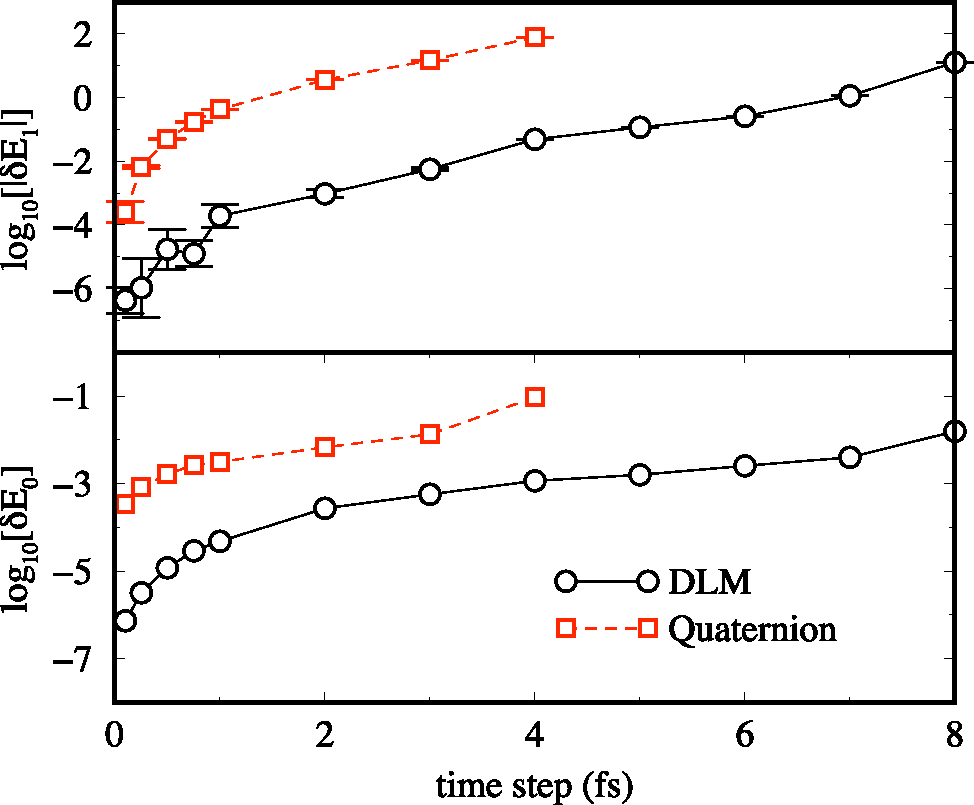
\includegraphics[width=\linewidth]{quatvsdlm.pdf}
\caption[Energy conservation analysis of the {\sc dlm} and quaternion 
integration methods]{Analysis of the energy conservation of the {\sc
dlm} and quaternion integration methods.  $\delta \mathrm{E}_1$ is the
linear drift in energy over time and $\delta \mathrm{E}_0$ is the
standard deviation of energy fluctuations around this drift.  All
simulations were of a 1024-molecule simulation of SSD water at 298 K
starting from the same initial configuration. Note that the {\sc dlm}
method provides more than an order of magnitude improvement in both
the energy drift and the size of the energy fluctuations when compared
with the quaternion method at any given time step.  At time steps
larger than 4 fs, the quaternion scheme resulted in rapidly rising
energies which eventually lead to simulation failure.  Using the {\sc
dlm} method, time steps up to 8 fs can be taken before this behavior
is evident.}
\label{quatdlm}
\end{figure}

In Fig.~\ref{quatdlm}, $\delta \mbox{E}_1$ is a measure of the linear
energy drift in units of $\mbox{kcal mol}^{-1}$ per particle over a
nanosecond of simulation time, and $\delta \mbox{E}_0$ is the standard
deviation of the energy fluctuations in units of $\mbox{kcal
mol}^{-1}$ per particle. In the top plot, it is apparent that the
energy drift is reduced by a significant amount (2 to 3 orders of
magnitude improvement at all tested time steps) by chosing the {\sc
dlm} method over the simple non-symplectic quaternion integration
method.  In addition to this improvement in energy drift, the
fluctuations in the total energy are also dampened by 1 to 2 orders of
magnitude by utilizing the {\sc dlm} method.

Although the {\sc dlm} method is more computationally expensive than
the traditional quaternion scheme for propagating a single time step,
consideration of the computational cost for a long simulation with a
particular level of energy conservation is in order.  A plot of energy
drift versus computational cost was generated
(Fig.~\ref{cpuCost}). This figure provides an estimate of the CPU time
required under the two integration schemes for 1 nanosecond of
simulation time for the model 1024-molecule system.  By chosing a
desired energy drift value it is possible to determine the CPU time
required for both methods. If a $\delta \mbox{E}_1$ of $1 \times
10^{-3} \mbox{kcal mol}^{-1}$ per particle is desired, a nanosecond of
simulation time will require ~19 hours of CPU time with the {\sc dlm}
integrator, while the quaternion scheme will require ~154 hours of CPU
time. This demonstrates the computational advantage of the integration
scheme utilized in {\sc oopse}.

\begin{figure}
\centering
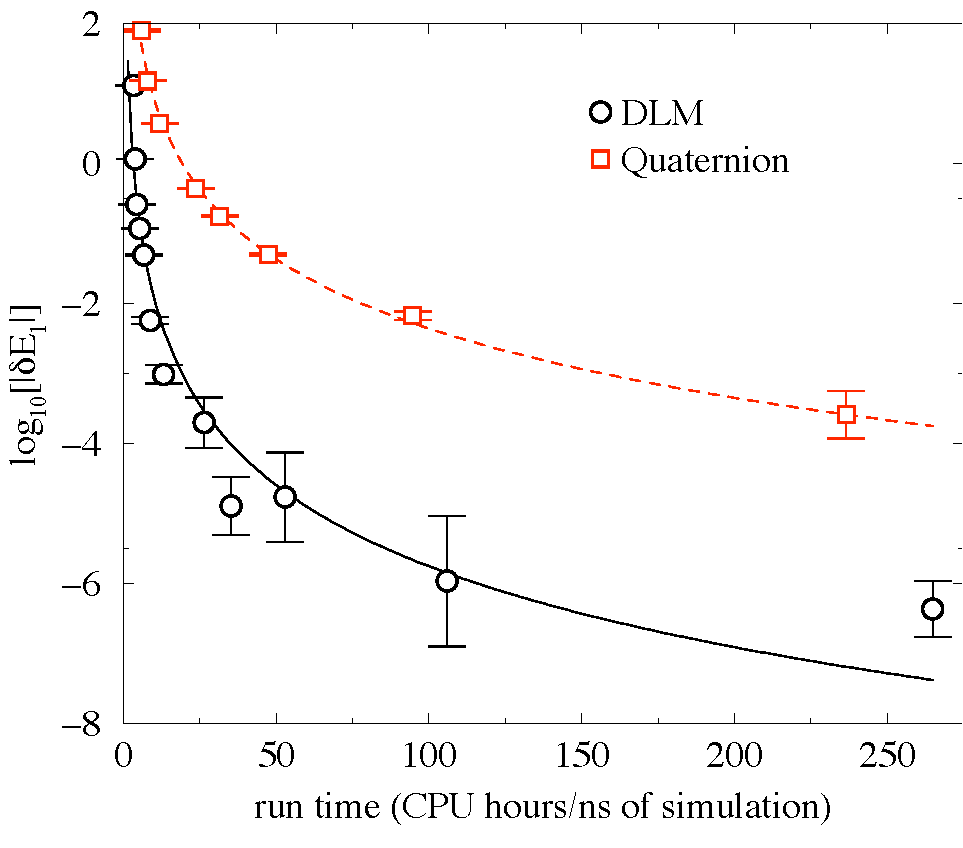
\includegraphics[width=\linewidth]{compCost.pdf}
\caption[Energy drift as a function of required simulation run 
time]{Energy drift as a function of required simulation run time.
$\delta \mathrm{E}_1$ is the linear drift in energy over time.
Simulations were performed on a single 2.5 GHz Pentium 4
processor. Simulation time comparisons can be made by tracing
horizontally from one curve to the other. For example, a simulation
that takes ~24 hours using the {\sc dlm} method will take roughly 210
hours using the simple quaternion method if the same degree of energy
conservation is desired.}
\label{cpuCost}
\end{figure}

There is only one specific keyword relevant to the default integrator,
and that is the time step for integrating the equations of motion.

\begin{center}
\begin{tabular}{llll}
{\bf variable} & {\bf Meta-data keyword} & {\bf units} & {\bf
default value} \\  
$h$ & {\tt dt = 2.0;} & fs & none 
\end{tabular}
\end{center}

\section{\label{sec:extended}Extended Systems for other Ensembles}

{\sc oopse} implements a number of extended system integrators for
sampling from other ensembles relevant to chemical physics.  The
integrator can be selected with the {\tt ensemble} keyword in the
meta-data file:

\begin{center}
\begin{tabular}{lll}
{\bf Integrator} & {\bf Ensemble} & {\bf Meta-data instruction} \\
NVE & microcanonical & {\tt ensemble = NVE; } \\
NVT & canonical & {\tt ensemble = NVT; } \\
NPTi & isobaric-isothermal & {\tt ensemble = NPTi;} \\
  &  (with isotropic volume changes) & \\
NPTf & isobaric-isothermal & {\tt ensemble = NPTf;} \\
  & (with changes to box shape) & \\
NPTxyz & approximate isobaric-isothermal & {\tt ensemble = NPTxyz;} \\
 &  (with separate barostats on each box dimension) & \\
\end{tabular}
\end{center}

The relatively well-known Nos\'e-Hoover thermostat\cite{Hoover85} is
implemented in {\sc oopse}'s NVT integrator.  This method couples an
extra degree of freedom (the thermostat) to the kinetic energy of the
system and it has been shown to sample the canonical distribution in
the system degrees of freedom while conserving a quantity that is, to
within a constant, the Helmholtz free energy.\cite{melchionna93}

NPT algorithms attempt to maintain constant pressure in the system by
coupling the volume of the system to a barostat.  {\sc oopse} contains
three different constant pressure algorithms.  The first two, NPTi and
NPTf have been shown to conserve a quantity that is, to within a
constant, the Gibbs free energy.\cite{melchionna93} The Melchionna
modification to the Hoover barostat is implemented in both NPTi and
NPTf.  NPTi allows only isotropic changes in the simulation box, while
box {\it shape} variations are allowed in NPTf.  The NPTxyz integrator
has {\it not} been shown to sample from the isobaric-isothermal
ensemble.  It is useful, however, in that it maintains orthogonality
for the axes of the simulation box while attempting to equalize
pressure along the three perpendicular directions in the box.

Each of the extended system integrators requires additional keywords
to set target values for the thermodynamic state variables that are
being held constant.  Keywords are also required to set the
characteristic decay times for the dynamics of the extended
variables.

\begin{center}
\begin{tabular}{llll}
{\bf variable} & {\bf Meta-data instruction} & {\bf units} & {\bf
default value} \\  
$T_{\mathrm{target}}$ & {\tt targetTemperature = 300;} &  K & none \\
$P_{\mathrm{target}}$ & {\tt targetPressure = 1;} & atm & none \\
$\tau_T$ & {\tt tauThermostat = 1e3;} & fs & none \\
$\tau_B$ & {\tt tauBarostat = 5e3;} & fs  & none \\
         & {\tt resetTime = 200;} & fs & none \\
         & {\tt useInitialExtendedSystemState = true;} & logical &
true
\end{tabular}
\end{center}

Two additional keywords can be used to either clear the extended
system variables periodically ({\tt resetTime}), or to maintain the
state of the extended system variables between simulations ({\tt
useInitialExtendedSystemState}).  More details on these variables
and their use in the integrators follows below.

\section{\label{oopseSec:noseHooverThermo}Nos\'{e}-Hoover Thermostatting}

The Nos\'e-Hoover equations of motion are given by\cite{Hoover85}
\begin{eqnarray}
\dot{{\bf r}} & = & {\bf v}, \\
\dot{{\bf v}} & = & \frac{{\bf f}}{m} - \chi {\bf v} ,\\
\dot{\mathsf{A}} & = & \mathsf{A} \cdot
\mbox{ skew}\left(\overleftrightarrow{\mathsf{I}}^{-1} \cdot {\bf j}\right), \\
\dot{{\bf j}} & = & {\bf j} \times \left( \overleftrightarrow{\mathsf{I}}^{-1}
\cdot {\bf j} \right) - \mbox{ rot}\left(\mathsf{A}^{T} \cdot \frac{\partial
V}{\partial \mathsf{A}} \right) - \chi {\bf j}.
\label{eq:nosehoovereom}
\end{eqnarray}

$\chi$ is an ``extra'' variable included in the extended system, and
it is propagated using the first order equation of motion
\begin{equation}
\dot{\chi} = \frac{1}{\tau_{T}^2} \left( \frac{T}{T_{\mathrm{target}}} - 1 \right).
\label{eq:nosehooverext}
\end{equation}

The instantaneous temperature $T$ is proportional to the total kinetic
energy (both translational and orientational) and is given by
\begin{equation}
T = \frac{2 K}{f k_B}
\end{equation}
Here, $f$ is the total number of degrees of freedom in the system,
\begin{equation}
f = 3 N + 2 N_{\mathrm{linear}} + 3 N_{\mathrm{non-linear}} - N_{\mathrm{constraints}},
\end{equation}
and $K$ is the total kinetic energy,
\begin{equation}
K = \sum_{i=1}^{N} \frac{1}{2} m_i {\bf v}_i^T \cdot {\bf v}_i +
\sum_{i=1}^{N_{\mathrm{linear}}+N_{\mathrm{non-linear}}}  \frac{1}{2} {\bf j}_i^T \cdot
\overleftrightarrow{\mathsf{I}}_i^{-1} \cdot {\bf j}_i.
\end{equation}
$N_{\mathrm{linear}}$ is the number of linear rotors (i.e. with two
non-zero moments of inertia), and $N_{\mathrm{non-linear}}$ is the
number of non-linear rotors (i.e. with three non-zero moments of
inertia).  

In eq.(\ref{eq:nosehooverext}), $\tau_T$ is the time constant for
relaxation of the temperature to the target value.  To set values for
$\tau_T$ or $T_{\mathrm{target}}$ in a simulation, one would use the
{\tt tauThermostat} and {\tt targetTemperature} keywords in the
meta-data file.  The units for {\tt tauThermostat} are fs, and the
units for the {\tt targetTemperature} are degrees K.   The integration
of the equations of motion is carried out in a velocity-Verlet style 2
part algorithm:

{\tt moveA:}
\begin{align*}
T(t) &\leftarrow \left\{{\bf v}(t)\right\}, \left\{{\bf j}(t)\right\} ,\\
%
{\bf v}\left(t + h / 2\right)  &\leftarrow {\bf v}(t) 
	+ \frac{h}{2} \left( \frac{{\bf f}(t)}{m} - {\bf v}(t)
	\chi(t)\right), \\
%
{\bf r}(t + h) &\leftarrow {\bf r}(t) 
	+ h {\bf v}\left(t + h / 2 \right) ,\\
%
{\bf j}\left(t + h / 2 \right)  &\leftarrow {\bf j}(t) 
	+ \frac{h}{2} \left( {\bf \tau}^b(t) - {\bf j}(t)
	\chi(t) \right) ,\\
%
\mathsf{A}(t + h) &\leftarrow \mathrm{rotate}
	\left(h * {\bf j}(t + h / 2) 
	\overleftrightarrow{\mathsf{I}}^{-1} \right) ,\\
%
\chi\left(t + h / 2 \right) &\leftarrow \chi(t) 
	+ \frac{h}{2 \tau_T^2} \left( \frac{T(t)}
	{T_{\mathrm{target}}} - 1 \right) .
\end{align*}

Here $\mathrm{rotate}(h * {\bf j}
\overleftrightarrow{\mathsf{I}}^{-1})$ is the same symplectic Trotter
factorization of the three rotation operations that was discussed in
the section on the {\sc dlm} integrator.  Note that this operation modifies
both the rotation matrix $\mathsf{A}$ and the angular momentum ${\bf
j}$.  {\tt moveA} propagates velocities by a half time step, and
positional degrees of freedom by a full time step.  The new positions
(and orientations) are then used to calculate a new set of forces and
torques in exactly the same way they are calculated in the {\tt
doForces} portion of the {\sc dlm} integrator.

Once the forces and torques have been obtained at the new time step,
the temperature, velocities, and the extended system variable can be
advanced to the same time value.

{\tt moveB:}
\begin{align*}
T(t + h) &\leftarrow \left\{{\bf v}(t + h)\right\}, 
	\left\{{\bf j}(t + h)\right\}, \\
%
\chi\left(t + h \right) &\leftarrow \chi\left(t + h /
	2 \right) + \frac{h}{2 \tau_T^2} \left( \frac{T(t+h)}
	{T_{\mathrm{target}}} - 1 \right), \\
%
{\bf v}\left(t + h \right)  &\leftarrow {\bf v}\left(t 
	+ h / 2 \right) + \frac{h}{2} \left(
	\frac{{\bf f}(t + h)}{m} - {\bf v}(t + h)
	\chi(t h)\right) ,\\
%
{\bf j}\left(t + h \right) &\leftarrow {\bf j}\left(t
	+ h / 2 \right) + \frac{h}{2} 
	\left( {\bf \tau}^b(t + h) - {\bf j}(t + h) 
	\chi(t + h) \right) .
\end{align*}

Since ${\bf v}(t + h)$ and ${\bf j}(t + h)$ are required to calculate
$T(t + h)$ as well as $\chi(t + h)$, they indirectly depend on their
own values at time $t + h$.  {\tt moveB} is therefore done in an
iterative fashion until $\chi(t + h)$ becomes self-consistent.  The
relative tolerance for the self-consistency check defaults to a value
of $\mbox{10}^{-6}$, but {\sc oopse} will terminate the iteration
after 4 loops even if the consistency check has not been satisfied.

The Nos\'e-Hoover algorithm is known to conserve a Hamiltonian for the
extended system that is, to within a constant, identical to the
Helmholtz free energy,\cite{melchionna93}
\begin{equation}
H_{\mathrm{NVT}} = V + K + f k_B T_{\mathrm{target}} \left(
\frac{\tau_{T}^2 \chi^2(t)}{2} + \int_{0}^{t} \chi(t^\prime) dt^\prime
\right).
\end{equation}
Poor choices of $h$ or $\tau_T$ can result in non-conservation
of $H_{\mathrm{NVT}}$, so the conserved quantity is maintained in the
last column of the {\tt .stat} file to allow checks on the quality of
the integration.

Bond constraints are applied at the end of both the {\tt moveA} and
{\tt moveB} portions of the algorithm.  Details on the constraint
algorithms are given in section \ref{oopseSec:rattle}.

\section{\label{sec:NPTi}Constant-pressure integration with 
isotropic box deformations (NPTi)}

To carry out isobaric-isothermal ensemble calculations, {\sc oopse}
implements the Melchionna modifications to the Nos\'e-Hoover-Andersen
equations of motion.\cite{melchionna93} The equations of motion are
the same as NVT with the following exceptions:

\begin{eqnarray}
\dot{{\bf r}} & = & {\bf v} + \eta \left( {\bf r} - {\bf R}_0 \right), \\
\dot{{\bf v}} & = & \frac{{\bf f}}{m} - (\eta + \chi) {\bf v}, \\
\dot{\eta} & = & \frac{1}{\tau_{B}^2 f k_B T_{\mathrm{target}}} V \left( P -
P_{\mathrm{target}} \right), \\
\dot{\mathcal{V}} & = & 3 \mathcal{V} \eta .
\label{eq:melchionna1}
\end{eqnarray}

$\chi$ and $\eta$ are the ``extra'' degrees of freedom in the extended
system.  $\chi$ is a thermostat, and it has the same function as it
does in the Nos\'e-Hoover NVT integrator.  $\eta$ is a barostat which
controls changes to the volume of the simulation box.  ${\bf R}_0$ is
the location of the center of mass for the entire system, and
$\mathcal{V}$ is the volume of the simulation box.  At any time, the
volume can be calculated from the determinant of the matrix which
describes the box shape:
\begin{equation}
\mathcal{V} = \det(\mathsf{H}).
\end{equation}

The NPTi integrator requires an instantaneous pressure. This quantity
is calculated via the pressure tensor,
\begin{equation}
\overleftrightarrow{\mathsf{P}}(t) = \frac{1}{\mathcal{V}(t)} \left(
\sum_{i=1}^{N} m_i {\bf v}_i(t) \otimes {\bf v}_i(t) \right) +
\overleftrightarrow{\mathsf{W}}(t).
\end{equation}
The kinetic contribution to the pressure tensor utilizes the {\it
outer} product of the velocities, denoted by the $\otimes$ symbol.  The
stress tensor is calculated from another outer product of the
inter-atomic separation vectors (${\bf r}_{ij} = {\bf r}_j - {\bf
r}_i$) with the forces between the same two atoms,
\begin{equation}
\overleftrightarrow{\mathsf{W}}(t) = \sum_{i} \sum_{j>i} {\bf r}_{ij}(t)
\otimes {\bf f}_{ij}(t).
\end{equation}
In systems containing cutoff groups, the stress tensor is computed
between the centers-of-mass of the cutoff groups:
\begin{equation}
\overleftrightarrow{\mathsf{W}}(t) = \sum_{a} \sum_{b} {\bf r}_{ab}(t)
\otimes {\bf f}_{ab}(t).
\end{equation}
where ${\bf r}_{ab}$ is the distance between the centers of mass, and 
\begin{equation}
{\bf f}_{ab} = s(r_{ab}) \sum_{i \in a} \sum_{j \in b} {\bf f}_{ij} +
s^{\prime}(r_{ab}) \frac{{\bf r}_{ab}}{|r_{ab}|} \sum_{i \in a} \sum_{j
\in b} V_{ij}({\bf r}_{ij}).
\end{equation}

The instantaneous pressure is then simply obtained from the trace of
the pressure tensor,
\begin{equation}
P(t) = \frac{1}{3} \mathrm{Tr} \left( \overleftrightarrow{\mathsf{P}}(t)
\right).
\end{equation}

In eq.(\ref{eq:melchionna1}), $\tau_B$ is the time constant for
relaxation of the pressure to the target value.  To set values for
$\tau_B$ or $P_{\mathrm{target}}$ in a simulation, one would use the
{\tt tauBarostat} and {\tt targetPressure} keywords in the meta-data
file.  The units for {\tt tauBarostat} are fs, and the units for the
{\tt targetPressure} are atmospheres.  Like in the NVT integrator, the
integration of the equations of motion is carried out in a
velocity-Verlet style two part algorithm with only the following
differences:

{\tt moveA:}
\begin{align*}
P(t) &\leftarrow \left\{{\bf r}(t)\right\}, \left\{{\bf v}(t)\right\} ,\\
%
{\bf v}\left(t + h / 2\right)  &\leftarrow {\bf v}(t) 
	+ \frac{h}{2} \left( \frac{{\bf f}(t)}{m} - {\bf v}(t)
	\left(\chi(t) + \eta(t) \right) \right), \\
%
\eta(t + h / 2) &\leftarrow \eta(t) + \frac{h 
	\mathcal{V}(t)}{2 N k_B T(t) \tau_B^2} \left( P(t) 
	- P_{\mathrm{target}} \right), \\ 
%
{\bf r}(t + h) &\leftarrow {\bf r}(t) + h 
	\left\{ {\bf v}\left(t + h / 2 \right) 
	+ \eta(t + h / 2)\left[ {\bf r}(t + h) 
	- {\bf R}_0 \right] \right\} ,\\
%
\mathsf{H}(t + h) &\leftarrow e^{-h \eta(t + h / 2)} 
	\mathsf{H}(t).
\end{align*}

The propagation of positions to time $t + h$
depends on the positions at the same time.  {\sc oopse} carries out
this step iteratively (with a limit of 5 passes through the iterative
loop).  Also, the simulation box $\mathsf{H}$ is scaled uniformly for
one full time step by an exponential factor that depends on the value
of $\eta$ at time $t +
h / 2$.  Reshaping the box uniformly also scales the volume of
the box by
\begin{equation}
\mathcal{V}(t + h) \leftarrow e^{ - 3 h \eta(t + h /2)} \times
\mathcal{V}(t).
\end{equation}

The {\tt doForces} step for the NPTi integrator is exactly the same as
in both the {\sc dlm} and NVT integrators.  Once the forces and torques have
been obtained at the new time step, the velocities can be advanced to
the same time value.

{\tt moveB:}
\begin{align*}
P(t + h) &\leftarrow  \left\{{\bf r}(t + h)\right\},
	\left\{{\bf v}(t + h)\right\}, \\
%
\eta(t + h) &\leftarrow \eta(t + h / 2) +
	\frac{h \mathcal{V}(t + h)}{2 N k_B T(t + h) 
	\tau_B^2} \left( P(t + h) - P_{\mathrm{target}} \right), \\ 
%
{\bf v}\left(t + h \right)  &\leftarrow {\bf v}\left(t 
	+ h / 2 \right) + \frac{h}{2} \left(
	\frac{{\bf f}(t + h)}{m} - {\bf v}(t + h)
	(\chi(t + h) + \eta(t + h)) \right) ,\\
%
{\bf j}\left(t + h \right)  &\leftarrow {\bf j}\left(t 
	+ h / 2 \right) + \frac{h}{2} \left( {\bf
	\tau}^b(t + h) - {\bf j}(t + h)
	\chi(t + h) \right) .
\end{align*}

Once again, since ${\bf v}(t + h)$ and ${\bf j}(t + h)$ are required
to calculate $T(t + h)$, $P(t + h)$, $\chi(t + h)$, and $\eta(t +
h)$, they indirectly depend on their own values at time $t + h$.  {\tt
moveB} is therefore done in an iterative fashion until $\chi(t + h)$
and $\eta(t + h)$ become self-consistent.  The relative tolerance for
the self-consistency check defaults to a value of $\mbox{10}^{-6}$,
but {\sc oopse} will terminate the iteration after 4 loops even if the
consistency check has not been satisfied.

The Melchionna modification of the Nos\'e-Hoover-Andersen algorithm is
known to conserve a Hamiltonian for the extended system that is, to
within a constant, identical to the Gibbs free energy,
\begin{equation}
H_{\mathrm{NPTi}} = V + K + f k_B T_{\mathrm{target}} \left(
\frac{\tau_{T}^2 \chi^2(t)}{2} + \int_{0}^{t} \chi(t^\prime) dt^\prime
\right) + P_{\mathrm{target}} \mathcal{V}(t).
\end{equation}
Poor choices of $\delta t$, $\tau_T$, or $\tau_B$ can result in
non-conservation of $H_{\mathrm{NPTi}}$, so the conserved quantity is
maintained in the last column of the {\tt .stat} file to allow checks
on the quality of the integration.  It is also known that this
algorithm samples the equilibrium distribution for the enthalpy
(including contributions for the thermostat and barostat), 
\begin{equation}
H_{\mathrm{NPTi}} = V + K + \frac{f k_B T_{\mathrm{target}}}{2} \left(
\chi^2 \tau_T^2 + \eta^2 \tau_B^2 \right) +  P_{\mathrm{target}}
\mathcal{V}(t). 
\end{equation}

Bond constraints are applied at the end of both the {\tt moveA} and
{\tt moveB} portions of the algorithm.  Details on the constraint
algorithms are given in section \ref{oopseSec:rattle}.

\section{\label{sec:NPTf}Constant-pressure integration with a
flexible box (NPTf)} 

There is a relatively simple generalization of the
Nos\'e-Hoover-Andersen method to include changes in the simulation box
{\it shape} as well as in the volume of the box.  This method utilizes
the full $3 \times 3$ pressure tensor and introduces a tensor of
extended variables ($\overleftrightarrow{\eta}$) to control changes to
the box shape.  The equations of motion for this method differ from
those of NPTi as follows:
\begin{eqnarray}
\dot{{\bf r}} & = & {\bf v} + \overleftrightarrow{\eta} \cdot \left( {\bf r} - {\bf R}_0 \right), \\
\dot{{\bf v}} & = & \frac{{\bf f}}{m} - (\overleftrightarrow{\eta} +
\chi \cdot \mathsf{1}) {\bf v}, \\
\dot{\overleftrightarrow{\eta}} & = & \frac{1}{\tau_{B}^2 f k_B
T_{\mathrm{target}}} V \left( \overleftrightarrow{\mathsf{P}} - P_{\mathrm{target}}\mathsf{1} \right) ,\\
\dot{\mathsf{H}} & = &  \overleftrightarrow{\eta} \cdot \mathsf{H} .
\label{eq:melchionna2}
\end{eqnarray}

Here, $\mathsf{1}$ is the unit matrix and $\overleftrightarrow{\mathsf{P}}$
is the pressure tensor.  Again, the volume, $\mathcal{V} = \det
\mathsf{H}$. 

The propagation of the equations of motion is nearly identical to the
NPTi integration:

{\tt moveA:}
\begin{align*}
\overleftrightarrow{\mathsf{P}}(t) &\leftarrow \left\{{\bf r}(t)\right\}, 
	\left\{{\bf v}(t)\right\} ,\\
%
{\bf v}\left(t + h / 2\right)  &\leftarrow {\bf v}(t) 
	+ \frac{h}{2} \left( \frac{{\bf f}(t)}{m} - 
	\left(\chi(t)\mathsf{1} + \overleftrightarrow{\eta}(t) \right) \cdot
	{\bf v}(t) \right), \\ 
%
\overleftrightarrow{\eta}(t + h / 2) &\leftarrow 
	\overleftrightarrow{\eta}(t) + \frac{h \mathcal{V}(t)}{2 N k_B
	T(t) \tau_B^2} \left( \overleftrightarrow{\mathsf{P}}(t) 
	- P_{\mathrm{target}}\mathsf{1} \right), \\ 
%
{\bf r}(t + h) &\leftarrow {\bf r}(t) + h \left\{ {\bf v}
	\left(t + h / 2 \right) + \overleftrightarrow{\eta}(t +
	h / 2) \cdot \left[ {\bf r}(t + h) 
	- {\bf R}_0 \right] \right\}, \\
%
\mathsf{H}(t + h) &\leftarrow \mathsf{H}(t) \cdot e^{-h
	\overleftrightarrow{\eta}(t + h / 2)} .
\end{align*}
{\sc oopse} uses a power series expansion truncated at second order
for the exponential operation which scales the simulation box.

The {\tt moveB} portion of the algorithm is largely unchanged from the
NPTi integrator:

{\tt moveB:}
\begin{align*}
\overleftrightarrow{\mathsf{P}}(t + h) &\leftarrow \left\{{\bf r}
	(t + h)\right\}, \left\{{\bf v}(t 
	+ h)\right\}, \left\{{\bf f}(t + h)\right\} ,\\
%
\overleftrightarrow{\eta}(t + h) &\leftarrow 
	\overleftrightarrow{\eta}(t + h / 2) +
	\frac{h \mathcal{V}(t + h)}{2 N k_B T(t + h) 
	\tau_B^2} \left( \overleftrightarrow{P}(t + h) 
	- P_{\mathrm{target}}\mathsf{1} \right) ,\\ 
%
{\bf v}\left(t + h \right)  &\leftarrow {\bf v}\left(t 
	+ h / 2 \right) + \frac{h}{2} \left(
	\frac{{\bf f}(t + h)}{m} - 
	(\chi(t + h)\mathsf{1} + \overleftrightarrow{\eta}(t 
	+ h)) \right) \cdot {\bf v}(t + h), \\
\end{align*}

The iterative schemes for both {\tt moveA} and {\tt moveB} are
identical to those described for the NPTi integrator.

The NPTf integrator is known to conserve the following Hamiltonian:
\begin{equation}
H_{\mathrm{NPTf}} = V + K + f k_B T_{\mathrm{target}} \left(
\frac{\tau_{T}^2 \chi^2(t)}{2} + \int_{0}^{t} \chi(t^\prime) dt^\prime
\right) + P_{\mathrm{target}} \mathcal{V}(t) + \frac{f k_B
T_{\mathrm{target}}}{2}
\mathrm{Tr}\left[\overleftrightarrow{\eta}(t)\right]^2 \tau_B^2.
\end{equation}

This integrator must be used with care, particularly in liquid
simulations.  Liquids have very small restoring forces in the
off-diagonal directions, and the simulation box can very quickly form
elongated and sheared geometries which become smaller than the cutoff
radius.  The NPTf integrator finds most use in simulating crystals or
liquid crystals which assume non-orthorhombic geometries.

\section{\label{nptxyz}Constant pressure in 3 axes (NPTxyz)}

There is one additional extended system integrator which is somewhat
simpler than the NPTf method described above.  In this case, the three
axes have independent barostats which each attempt to preserve the
target pressure along the box walls perpendicular to that particular
axis.  The lengths of the box axes are allowed to fluctuate
independently, but the angle between the box axes does not change.
The equations of motion are identical to those described above, but
only the {\it diagonal} elements of $\overleftrightarrow{\eta}$ are
computed.  The off-diagonal elements are set to zero (even when the
pressure tensor has non-zero off-diagonal elements).

It should be noted that the NPTxyz integrator is {\it not} known to
preserve any Hamiltonian of interest to the chemical physics
community.  The integrator is extremely useful, however, in generating
initial conditions for other integration methods.  It {\it is} suitable
for use with liquid simulations, or in cases where there is
orientational anisotropy in the system (i.e. in lipid bilayer
simulations).


\section{\label{sec:constraints}Constraint Methods}

\subsection{\label{oopseSec:rattle}The {\sc rattle} Method for Bond 
	Constraints}

In order to satisfy the constraints of fixed bond lengths within {\sc
oopse}, we have implemented the {\sc rattle} algorithm of
Andersen.\cite{andersen83} {\sc rattle} is a velocity-Verlet
formulation of the {\sc shake} method\cite{ryckaert77} for iteratively
solving the Lagrange multipliers which maintain the holonomic
constraints.  Both methods are covered in depth in the
literature,\cite{leach01:mm,Allen87} and a detailed description of
this method would be redundant.

\subsection{\label{oopseSec:zcons}The Z-Constraint Method}

A force auto-correlation method based on the fluctuation-dissipation
theorem was developed by Roux and Karplus to investigate the dynamics
of ions inside ion channels.\cite{Roux91} The time-dependent friction
coefficient can be calculated from the deviation of the instantaneous
force from its mean value:
\begin{equation}
\xi(z,t)=\langle\delta F(z,t)\delta F(z,0)\rangle/k_{B}T,
\end{equation}
where%
\begin{equation}
\delta F(z,t)=F(z,t)-\langle F(z,t)\rangle.
\end{equation}

If the time-dependent friction decays rapidly, the static friction
coefficient can be approximated by
\begin{equation}
\xi_{\text{static}}(z)=\int_{0}^{\infty}\langle\delta F(z,t)\delta F(z,0)\rangle dt.
\end{equation}

This allows the diffusion constant to then be calculated through the
Einstein relation:\cite{Marrink94}
\begin{equation}
D(z)=\frac{k_{B}T}{\xi_{\text{static}}(z)}=\frac{(k_{B}T)^{2}}{\int_{0}^{\infty
}\langle\delta F(z,t)\delta F(z,0)\rangle dt}.%
\end{equation}

The Z-Constraint method, which fixes the $z$ coordinates of a few
``tagged'' molecules with respect to the center of the mass of the
system is a technique that was proposed to obtain the forces required
for the force auto-correlation calculation.\cite{Marrink94} However,
simply resetting the coordinate will move the center of the mass of
the whole system. To avoid this problem, we have developed a new
method that is utilized in {\sc oopse}. Instead of resetting the
coordinates, we reset the forces of $z$-constrained molecules and
subtract the total constraint forces from the rest of the system after
the force calculation at each time step.

After the force calculation, the total force on molecule $\alpha$ is:
\begin{equation}
G_{\alpha} = \sum_i F_{\alpha i},
\label{oopseEq:zc1}
\end{equation}
where $F_{\alpha i}$ is the force in the $z$ direction on atom $i$ in
$z$-constrained molecule $\alpha$. The forces on the atoms in the
$z$-constrained molecule are then adjusted to remove the total force
on molecule $\alpha$:
\begin{equation}
F_{\alpha i} = F_{\alpha i} - 
	\frac{m_{\alpha i} G_{\alpha}}{\sum_i m_{\alpha i}}.
\end{equation}
Here, $m_{\alpha i}$ is the mass of atom $i$ in the $z$-constrained
molecule.  After the forces have been adjusted, the velocities must
also be modified to subtract out molecule $\alpha$'s center-of-mass
velocity in the $z$ direction.
\begin{equation}
v_{\alpha i} = v_{\alpha i} -
	\frac{\sum_i m_{\alpha i} v_{\alpha i}}{\sum_i m_{\alpha i}},
\end{equation}
where $v_{\alpha i}$ is the velocity of atom $i$ in the $z$ direction.
Lastly, all of the accumulated constraint forces must be subtracted
from the rest of the unconstrained system to keep the system center of
mass of the entire system from drifting.
\begin{equation}
F_{\beta i} = F_{\beta i} - \frac{m_{\beta i} \sum_{\alpha} G_{\alpha}}
	{\sum_{\beta}\sum_i m_{\beta i}},
\end{equation}
where $\beta$ denotes all {\it unconstrained} molecules in the
system. Similarly, the velocities of the unconstrained molecules must
also be scaled:
\begin{equation}
v_{\beta i} = v_{\beta i} + \sum_{\alpha} \frac{\sum_i m_{\alpha i}
v_{\alpha i}}{\sum_i m_{\alpha i}}.
\end{equation}

This method will pin down the centers-of-mass of all of the
$z$-constrained molecules, and will also keep the entire system fixed
at the original system center-of-mass location.

At the very beginning of the simulation, the molecules may not be at
their desired positions. To steer a $z$-constrained molecule to its
specified position, a simple harmonic potential is used:
\begin{equation}
U(t)=\frac{1}{2}k_{\text{Harmonic}}(z(t)-z_{\text{cons}})^{2},%
\end{equation}
where $k_{\text{Harmonic}}$ is an harmonic force constant, $z(t)$ is
the current $z$ coordinate of the center of mass of the constrained
molecule, and $z_{\text{cons}}$ is the desired constraint
position. The harmonic force operating on the $z$-constrained molecule
at time $t$ can be calculated by
\begin{equation}
F_{z_{\text{Harmonic}}}(t)=-\frac{\partial U(t)}{\partial z(t)}=
	-k_{\text{Harmonic}}(z(t)-z_{\text{cons}}).
\end{equation}

The user may also specify the use of a constant velocity method
(steered molecular dynamics) to move the molecules to their desired
initial positions. Based on concepts from atomic force microscopy,
{\sc smd} has been used to study many processes which occur via rare
events on the time scale of a few hundreds of picoseconds.  For
example,{\sc smd} has been used to observe the dissociation of
Streptavidin-biotin Complex.\cite{smd}  

To use of the $z$-constraint method in an {\sc oopse} simulation, the
molecules must be specified using the {\tt nZconstraints} keyword in
the meta-data file.  The other parameters for modifying the behavior
of the $z$-constraint method are listed in table~\ref{table:zconParams}.

\begin{longtable}[c]{ABCD}
\caption{Meta-data Keywords: Z-Constraint Parameters}
\\
{\bf keyword} & {\bf units} & {\bf use} & {\bf remarks}  \\ \hline
\endhead
\hline
\endfoot
{\tt zconsTime} & fs & Sets the frequency at which the {\tt .fz} file
is written &  \\ 
{\tt zconsForcePolicy} & string & The strategy for subtracting
the $z$-constraint force from the {\it unconstrained} molecules & Possible
strategies are {\tt BYMASS} and {\tt BYNUMBER}. The default
strategy is {\tt BYMASS}\\ 
{\tt zconsGap} & $\mbox{\AA}$ & Sets the distance between two adjacent
constraint positions&Used mainly to move molecules through a
simulation to estimate potentials of mean force. \\ 
{\tt zconsFixtime} & fs & Sets the length of time the $z$-constraint
molecule is held fixed & {\tt zconsFixtime} must be set if {\tt
zconsGap} is set\\ 
{\tt zconsUsingSMD} & logical & Flag for using Steered Molecular
Dynamics to move the molecules to the correct constrained positions  &
Harmonic Forces are used by default
\label{table:zconParams}
\end{longtable}

\section{Langevin Dynamics for Rigid Particles of Arbitrary Shape (LANGEVINDYNAMICS)\label{LDRB}}

{\sc oopse} implements langevin dynamics integrator to perform the
molecular dynamics simulations at implicit solvents environment to
speed up the simulation when the properties of solvents are not
important. Consider the Langevin equations of motion in generalized
coordinates
\begin{equation}
{\bf M} \dot{{\bf V}}(t) = {\bf F}_{s}(t) +
{\bf F}_{f}(t)  + {\bf F}_{r}(t) 
\label{LDGeneralizedForm}
\end{equation}
where ${\bf M}$ is a $6 \times 6$ diagonal mass matrix (which
includes the mass of the rigid body as well as the moments of inertia
in the body-fixed frame) and ${\bf V}$ is a generalized velocity,
${\bf V} =
\left\{{\bf v},{\bf \omega}\right\}$. The right side of
Eq.~\ref{LDGeneralizedForm} consists of three generalized forces: a
system force (${\bf F}_{s}$), a frictional or dissipative force (${\bf
F}_{f}$) and a stochastic force (${\bf F}_{r}$). While the evolution
of the system in Newtonian mechanics is typically done in the lab
frame, it is convenient to handle the dynamics of rigid bodies in
body-fixed frames. Thus the friction and random forces on each
substructure are calculated in a body-fixed frame and may converted
back to the lab frame using that substructure's rotation matrix (${\bf
Q}$):
\begin{equation}
{\bf F}_{f,r} = 
\left( \begin{array}{c}
{\bf f}_{f,r} \\
{\bf \tau}_{f,r}
\end{array} \right)
=
\left( \begin{array}{c}
{\bf Q}^{T} {\bf f}^{~b}_{f,r} \\
{\bf Q}^{T} {\bf \tau}^{~b}_{f,r}
\end{array} \right)
\end{equation}
The body-fixed friction force, ${\bf F}_{f}^{~b}$, is proportional to
the (body-fixed) velocity at the center of resistance
${\bf v}_{R}^{~b}$ and the angular velocity ${\bf \omega}$
\begin{equation}
{\bf F}_{f}^{~b}(t) = \left( \begin{array}{l}
 {\bf f}_{f}^{~b}(t) \\
 {\bf \tau}_{f}^{~b}(t) \\
 \end{array} \right) =  - \left( \begin{array}{*{20}c}
   \Xi_{R}^{tt} & \Xi_{R}^{rt} \\
   \Xi_{R}^{tr} & \Xi_{R}^{rr}    \\
\end{array} \right)\left( \begin{array}{l}
 {\bf v}_{R}^{~b}(t) \\
 {\bf \omega}(t) \\
 \end{array} \right),
\end{equation}
while the random force, ${\bf F}_{r}$, is a Gaussian stochastic
variable with zero mean and variance,
\begin{equation}
\left\langle {{\bf F}_{r}(t) ({\bf F}_{r}(t'))^T } \right\rangle  =
\left\langle {{\bf F}_{r}^{~b} (t) ({\bf F}_{r}^{~b} (t'))^T } \right\rangle  =
2 k_B T \Xi_R \delta(t - t'). \label{eq:randomForce}
\end{equation}
$\Xi_R$ is the $6\times6$ resistance tensor at the center of
resistance.  Once this tensor is known for a given rigid body (as
described in the previous section) obtaining a stochastic vector that
has the properties in Eq. (\ref{eq:randomForce}) can be done
efficiently by carrying out a one-time Cholesky decomposition to
obtain the square root matrix of the resistance tensor,
\begin{equation} 
\Xi_R = {\bf S} {\bf S}^{T},
\label{eq:Cholesky}
\end{equation} 
where ${\bf S}$ is a lower triangular matrix.\cite{Schlick2002} A
vector with the statistics required for the random force can then be
obtained by multiplying ${\bf S}$ onto a random 6-vector ${\bf Z}$ which
has elements chosen from a Gaussian distribution, such that:
\begin{equation}
\langle {\bf Z}_i \rangle = 0, \hspace{1in} \langle {\bf Z}_i \cdot
{\bf Z}_j \rangle = \frac{2 k_B T}{\delta t} \delta_{ij},
\end{equation}
where $\delta t$ is the timestep in use during the simulation. The
random force, ${\bf F}_{r}^{~b} = {\bf S} {\bf Z}$, can be shown to have the
correct properties required by Eq. (\ref{eq:randomForce}).

The equation of motion for the translational velocity of the center of
mass (${\bf v}$) can be written as
\begin{equation}
m \dot{{\bf v}} (t) =  {\bf f}_{s}(t) + {\bf f}_{f}(t) +
{\bf f}_{r}(t)
\end{equation}
Since the frictional and random forces are applied at the center of
resistance, which generally does not coincide with the center of mass,
extra torques are exerted at the center of mass. Thus, the net
body-fixed torque at the center of mass, $\tau^{~b}(t)$,
is given by
\begin{equation}
\tau^{~b} \leftarrow \tau_{s}^{~b} + \tau_{f}^{~b} + \tau_{r}^{~b} + {\bf r}_{MR} \times \left( {\bf f}_{f}^{~b} + {\bf f}_{r}^{~b} \right)
\end{equation}
where ${\bf r}_{MR}$ is the vector from the center of mass to the center of
resistance. Instead of integrating the angular velocity in lab-fixed
frame, we consider the equation of motion for the angular momentum
(${\bf j}$) in the body-fixed frame
\begin{equation}
\frac{\partial}{\partial t}{\bf j}(t) = \tau^{~b}(t)
\end{equation}
Embedding the friction and random forces into the the total force and
torque, one can integrate the Langevin equations of motion for a rigid
body of arbitrary shape in a velocity-Verlet style 2-part algorithm,
where $h = \delta t$:

{\tt move A:}
\begin{align*}
{\bf v}\left(t + h / 2\right)  &\leftarrow  {\bf v}(t)
    + \frac{h}{2} \left( {\bf f}(t) / m \right), \\
%
{\bf r}(t + h) &\leftarrow {\bf r}(t)
    + h  {\bf v}\left(t + h / 2 \right), \\
%
{\bf j}\left(t + h / 2 \right)  &\leftarrow {\bf j}(t)
    + \frac{h}{2} {\bf \tau}^{~b}(t), \\
%
{\bf Q}(t + h) &\leftarrow \mathrm{rotate}\left( h {\bf j}
    (t + h / 2) \cdot \overleftrightarrow{\mathsf{I}}^{-1} \right).
\end{align*}
In this context, $\overleftrightarrow{\mathsf{I}}$ is the diagonal
moment of inertia tensor, and the $\mathrm{rotate}$ function is the
reversible product of the three body-fixed rotations,
\begin{equation}
\mathrm{rotate}({\bf a}) = \mathsf{G}_x(a_x / 2) \cdot
\mathsf{G}_y(a_y / 2) \cdot \mathsf{G}_z(a_z) \cdot \mathsf{G}_y(a_y
/ 2) \cdot \mathsf{G}_x(a_x /2),
\end{equation}
where each rotational propagator, $\mathsf{G}_\alpha(\theta)$,
rotates both the rotation matrix ($\mathbf{Q}$) and the body-fixed
angular momentum (${\bf j}$) by an angle $\theta$ around body-fixed
axis $\alpha$,
\begin{equation}
\mathsf{G}_\alpha( \theta ) = \left\{
\begin{array}{lcl}
\mathbf{Q}(t) & \leftarrow & \mathbf{Q}(0) \cdot \mathsf{R}_\alpha(\theta)^T, \\
{\bf j}(t) & \leftarrow & \mathsf{R}_\alpha(\theta) \cdot {\bf
j}(0).
\end{array}
\right.
\end{equation}
$\mathsf{R}_\alpha$ is a quadratic approximation to the single-axis
rotation matrix.  For example, in the small-angle limit, the
rotation matrix around the body-fixed x-axis can be approximated as
\begin{equation}
\mathsf{R}_x(\theta) \approx \left(
\begin{array}{ccc}
1 & 0 & 0 \\
0 & \frac{1-\theta^2 / 4}{1 + \theta^2 / 4}  & -\frac{\theta}{1+
\theta^2 / 4} \\
0 & \frac{\theta}{1+ \theta^2 / 4} & \frac{1-\theta^2 / 4}{1 +
\theta^2 / 4}
\end{array}
\right).
\end{equation}
All other rotations follow in a straightforward manner. After the
first part of the propagation, the forces and body-fixed torques are
calculated at the new positions and orientations.  The system forces
and torques are derivatives of the total potential energy function
($U$) with respect to the rigid body positions (${\bf r}$) and the
columns of the transposed rotation matrix ${\bf Q}^T = \left({\bf
u}_x, {\bf u}_y, {\bf u}_z \right)$:

{\tt Forces:}
\begin{align*}
{\bf f}_{s}(t + h) & \leftarrow
    - \left(\frac{\partial U}{\partial {\bf r}}\right)_{{\bf r}(t + h)} \\
%
{\bf \tau}_{s}(t + h) &\leftarrow {\bf u}(t + h)
    \times \frac{\partial U}{\partial {\bf u}} \\
%
{\bf v}^{b}_{R}(t+h) & \leftarrow \mathbf{Q}(t+h) \cdot \left({\bf v}(t+h) + {\bf \omega}(t+h) \times {\bf r}_{MR} \right) \\
%
{\bf f}_{R,f}^{b}(t+h) & \leftarrow - \Xi_{R}^{tt} \cdot
{\bf v}^{b}_{R}(t+h) - \Xi_{R}^{rt} \cdot {\bf \omega}(t+h) \\
%
{\bf \tau}_{R,f}^{b}(t+h) & \leftarrow - \Xi_{R}^{tr} \cdot
{\bf v}^{b}_{R}(t+h) - \Xi_{R}^{rr} \cdot {\bf \omega}(t+h) \\
%
Z & \leftarrow  {\tt GaussianNormal}(2 k_B T / h, 6) \\
{\bf F}_{R,r}^{b}(t+h) & \leftarrow {\bf S} \cdot Z \\
%
{\bf f}(t+h) & \leftarrow {\bf f}_{s}(t+h) + \mathbf{Q}^{T}(t+h)
\cdot \left({\bf f}_{R,f}^{~b} + {\bf f}_{R,r}^{~b} \right) \\
%
\tau(t+h) & \leftarrow \tau_{s}(t+h) + \mathbf{Q}^{T}(t+h) \cdot \left(\tau_{R,f}^{~b} + \tau_{R,r}^{~b} \right) + {\bf r}_{MR} \times \left({\bf f}_{f}(t+h) + {\bf f}_{r}(t+h) \right) \\
\tau^{~b}(t+h) & \leftarrow \mathbf{Q}(t+h) \cdot \tau(t+h) \\
\end{align*}
Frictional (and random) forces and torques must be computed at the
center of resistance, so there are additional steps required to find
the body-fixed velocity (${\bf v}_{R}^{~b}$) at this location.  Mapping
the frictional and random forces at the center of resistance back to
the center of mass also introduces an additional term in the torque
one obtains at the center of mass.

Once the forces and torques have been obtained at the new time step,
the velocities can be advanced to the same time value.

{\tt move B:}
\begin{align*}
{\bf v}\left(t + h \right)  &\leftarrow  {\bf v}\left(t + h / 2
\right)
    + \frac{h}{2} \left( {\bf f}(t + h) / m \right), \\
%
{\bf j}\left(t + h \right)  &\leftarrow {\bf j}\left(t + h / 2
\right)
    + \frac{h}{2} {\bf \tau}^{~b}(t + h) .
\end{align*}

The viscosity of the implicit of solvents must be specified using {\tt
viscosity} keywords in the meta-data file to use langevin dynamics
integrator. For simple shaped particles (spheres and ellipsoids), no
further parameters are necessary. However, there are no analytical
solutions for composite shaped particles, the approximate methods have
to be applied to get the resistance tensor. The file which contains
the information about hydro properties is indicated by {\tt
HydroPropFile} keyword in meta-data file. The {\tt HydroPropFile} is
precalculated by {\tt Hydro}.

\begin{longtable}[c]{ABCD}
\caption{Meta-data Keywords: Langevin Dynamics Parameters}
\\
{\bf keyword} & {\bf units} & {\bf use} & {\bf remarks}  \\ \hline
\endhead
\hline
\endfoot
{\tt viscosity} & centipoise & Sets the value of viscosity of implicit
solvents & \\ {\tt HydroPropFile} & string & specifies the resistance
tensor file & usually a {\tt .diff} file which is precalculated by
{\sc Hydro}. Not necessory for simple shaped particles (spheres and
ellipsoids) \\ 
{\tt beadSize} & $\mbox{\AA}$ & Sets the diameters of
beads when {\sc Rough Shell Model} is used to generate the resistance
tensor file. \\
\label{table:ldParameters}
\end{longtable}

\chapter{\label{oopseSec:thermInt}Thermodynamic Integration}

Thermodynamic integration is an established technique that has been
used extensively in the calculation of free energies for condensed
phases of
materials.\cite{Frenkel84,Hermens88,Meijer90,Baez95a,Vlot99}.  This
method uses a sequence of simulations during which the system of
interest is converted into a reference system for which the free
energy is known analytically ($A_0$).  The difference in potential
energy between the reference system and the system of interest
($\Delta V$) is then integrated in order to determine the free energy
difference between the two states:
\begin{equation}
 A = A_0 + \int_0^1 \left\langle \Delta V \right\rangle_\lambda
d\lambda.
\label{eq:thermInt}
\end{equation}
Here, $\lambda$ is the parameter that governs the transformation
between the reference system and the system of interest.  For
crystalline phases, an harmonically-restrained (Einstein) crystal is
chosen as the reference state, while for liquid phases, the ideal gas
is taken as the reference state.  

In an Einstein crystal, the molecules are restrained at their ideal
lattice locations and orientations. Using harmonic restraints, as
applied by B\`{a}ez and Clancy, the total potential for this reference
crystal ($V_\mathrm{EC}$) is the sum of all the harmonic restraints,
\begin{equation}
V_\mathrm{EC} = \sum_{i} \left[ \frac{K_\mathrm{v}}{2} (r_i - r_i^\circ)^2 +
\frac{K_\theta}{2} (\theta_i - \theta_i^\circ)^2 +
\frac{K_\omega}{2}(\omega_i - \omega_i^\circ)^2 \right],
\end{equation}
where $K_\mathrm{v}$, $K_\mathrm{\theta}$, and $K_\mathrm{\omega}$ are
the spring constants restraining translational motion and deflection
of and rotation around the principle axis of the molecule
respectively.  The values of $\theta$ range from $0$ to $\pi$, while
$\omega$ ranges from $-\pi$ to $\pi$.

The partition function for a molecular crystal restrained in this
fashion can be evaluated analytically, and the Helmholtz Free Energy
({\it A}) is given by
\begin{eqnarray}
\frac{A}{N} = \frac{E_m}{N}\ -\ kT\ln \left (\frac{kT}{h\nu}\right )^3&-&kT\ln \left
[\pi^\frac{1}{2}\left (\frac{8\pi^2I_\mathrm{A}kT}{h^2}\right
)^\frac{1}{2}\left (\frac{8\pi^2I_\mathrm{B}kT}{h^2}\right
)^\frac{1}{2}\left (\frac{8\pi^2I_\mathrm{C}kT}{h^2}\right
)^\frac{1}{2}\right ] \nonumber \\ &-& kT\ln \left [\frac{kT}{2(\pi
K_\omega K_\theta)^{\frac{1}{2}}}\exp\left
(-\frac{kT}{2K_\theta}\right)\int_0^{\left (\frac{kT}{2K_\theta}\right
)^\frac{1}{2}}\exp(t^2)\mathrm{d}t\right ],
\label{ecFreeEnergy}
\end{eqnarray}
where $2\pi\nu = (K_\mathrm{v}/m)^{1/2}$, and $E_m$ is the minimum
potential energy of the ideal crystal.\cite{Baez95a} 

{\sc oopse} can perform the simulations that aid the user in
constructing the thermodynamic path from the molecular system to one
of the reference systems.  To do this, the user sets the value of
$\lambda$ (between 0 \& 1) in the meta-data file.  If the system of
interest is crystalline, {\sc oopse} must be able to find the  {\it
reference} configuration of the system in a file called {\tt
idealCrystal.in} in the directory from which the simulation was run.
This file is a standard {\tt .dump} file, but all information about
velocities and angular momenta are discarded when the file is read. 

The configuration found in the {\tt idealCrystal.in} file is used for 
the reference positions and molecular orientations of the Einstein
crystal.  To complete the specification of the Einstein crystal, a set
of force constants must also be specified; one for displacments of the
molecular centers of mass, and two for displacements from the ideal
orientations of the molecules.  

To construct a thermodynamic integration path, the user would run a
sequence of $N$ simulations, each with a different value of lambda
between $0$ and $1$.  When {\tt useSolidThermInt} is set to {\tt true}
in the meta-data file, two additional energy columns are reported in
the {\tt .stat} file for the simulation.  The first, {\tt vRaw}, is
the unperturbed energy for the configuration, and the second, {\tt
vHarm}, is the energy of the harmonic (Einstein) system in an
identical configuration.   The total potential energy of the
configuration is a linear combination of {\tt vRaw} and {\tt vHarm}
weighted by the value of $\lambda$.

From a running average of the difference between {\tt vRaw} and {\tt
vHarm}, the user can obtain the integrand in Eq. (\ref{eq:thermInt})
for fixed value of $\lambda$.  

There are two additional files with the suffixes {\tt .zang0} and {\tt
.zang} generated by {\sc oopse} during the first run of a solid
thermodynamic integration.  These files contain the initial ({\tt
.zang0}) and  final ({\tt .zang}) values of the angular displacement
coordinates for each of the molecules.  These are particularly useful
when chaining a number of simulations (with successive values of
$\lambda$) together.  

For {\it liquid} thermodynamic integrations, the reference system is
the ideal gas (with a potential exactly equal to 0), so the {\tt
.stat} file contains only the standard columns. The potential energy
column contains the potential of the {\it unperturbed} system (and not
the $\lambda$-weighted potential.  This allows the user to use the 
potential energy directly as the $\Delta V$ in the integrand of
Eq. (\ref{eq:thermInt}). 

Meta-data parameters concerning thermodynamic integrations are given in
Table~\ref{table:thermIntParams}

\begin{longtable}[c]{ABCD}
\caption{Meta-data Keywords: Thermodynamic Integration Parameters}
\\
{\bf keyword} & {\bf units} & {\bf use} & {\bf remarks}  \\ \hline
\endhead
\hline
\endfoot
{\tt useSolidThermInt} & logical & perform thermodynamic integration
to an Einstein crystal? & default is ``false'' \\
{\tt useLiquidThermInt} & logical & perform thermodynamic integration
to an ideal gas? & default is ``false'' \\
{\tt thermodynamicIntegrationLambda} & & & \\
 & double & transformation
parameter & Sets how far along the thermodynamic integration path the
simulation will be. \\
{\tt thermodynamicIntegrationK} & & & \\
 & double & & power of $\lambda$
governing shape of integration pathway \\
{\tt thermIntDistSpringConst} & & & \\
 & $\mbox{kcal~mol}^{-1} \mbox{\AA}^{-2}$
& & spring constant for translations in Einstein crystal \\
{\tt thermIntThetaSpringConst} & & & \\
 & $\mbox{kcal~mol}^{-1}
\mbox{rad}^{-2}$ & & spring constant for deflection away from z-axis
in Einstein crystal \\
{\tt thermIntOmegaSpringConst} & & &  \\
 & $\mbox{kcal~mol}^{-1}
\mbox{rad}^{-2}$ & & spring constant for rotation around z-axis in
Einstein crystal 
\label{table:thermIntParams}
\end{longtable}


\chapter{\label{oopseSec:minimizer}Energy Minimization}

As one of the basic procedures of molecular modeling, energy
minimization is used to identify local configurations that are stable
points on the potential energy surface. There is a vast literature on
energy minimization algorithms have been developed to search for the
global energy minimum as well as to find local structures which are
stable fixed points on the surface.  We have included two simple
minimization algorithms: steepest descent, ({\sc sd}) and conjugate
gradient ({\sc cg}) to help users find reasonable local minima from
their initial configurations. Since {\sc oopse} handles atoms and
rigid bodies which have orientational coordinates as well as
translational coordinates, there is some subtlety to the choice of
parameters for minimization algorithms.

Given a coordinate set $x_{k}$ and a search direction $d_{k}$, a line
search algorithm is performed along $d_{k}$ to produce
$x_{k+1}=x_{k}+$ $\lambda _{k}d_{k}$. In the steepest descent ({\sc
sd}) algorithm,%
\begin{equation}
d_{k}=-\nabla V(x_{k}).
\end{equation}
The gradient and the direction of next step are always orthogonal.
This may cause oscillatory behavior in narrow valleys.  To overcome
this problem, the Fletcher-Reeves variant~\cite{FletcherReeves} of the
conjugate gradient ({\sc cg}) algorithm is used to generate $d_{k+1}$
via simple recursion:
\begin{equation}
d_{k+1}  =-\nabla V(x_{k+1})+\gamma_{k}d_{k}
\end{equation}
where
\begin{equation}
\gamma_{k}  =\frac{\nabla V(x_{k+1})^{T}\nabla V(x_{k+1})}{\nabla
V(x_{k})^{T}\nabla V(x_{k})}.
\end{equation}

The Polak-Ribiere variant~\cite{PolakRibiere} of the conjugate
gradient ($\gamma_{k}$) is defined as%
\begin{equation}
\gamma_{k}=\frac{[\nabla V(x_{k+1})-\nabla V(x)]^{T}\nabla V(x_{k+1})}{\nabla
V(x_{k})^{T}\nabla V(x_{k})}%
\end{equation}
It is widely agreed that the Polak-Ribiere variant gives better
convergence than the Fletcher-Reeves variant, so the conjugate
gradient approach implemented in {\sc oopse} is the Polak-Ribiere
variant.

The conjugate gradient method assumes that the conformation is close
enough to a local minimum that the potential energy surface is very
nearly quadratic.  When the initial structure is far from the minimum,
the steepest descent method can be superior to the conjugate gradient
method. Hence, the steepest descent method is often used for the first
10-100 steps of minimization. Another useful feature of minimization
methods in {\sc oopse} is that a modified {\sc shake} algorithm can be
applied during the minimization to constraint the bond lengths if this
is required by the force field. Meta-data parameters concerning the
minimizer are given in Table~\ref{table:minimizeParams}

\begin{longtable}[c]{ABCD}
\caption{Meta-data Keywords: Energy Minimizer Parameters}
\\
{\bf keyword} & {\bf units} & {\bf use} & {\bf remarks}  \\ \hline
\endhead
\hline
\endfoot
{\tt minimizer} & string &  selects the minimization method to be used
& either {\tt CG} (conjugate gradient) or {\tt SD} (steepest
descent) \\ 
{\tt minimizerMaxIter} & steps & Sets the maximum number of iterations
for the energy minimization & The default value is 200\\
{\tt minimizerWriteFreq} & steps & Sets the frequency with which the {\tt .dump} and {\tt .stat} files are writtern during energy minimization & \\
{\tt minimizerStepSize} & $\mbox{\AA}$ &  Sets the step size for the
line search & The default value is 0.01\\
{\tt minimizerFTol} & $\mbox{kcal mol}^{-1}$  & Sets the energy tolerance
for stopping the minimziation. & The default value is $10^{-8}$\\
{\tt minimizerGTol} & $\mbox{kcal mol}^{-1}\mbox{\AA}^{-1}$ & Sets the
gradient tolerance for stopping the minimization. & The default value
is  $10^{-8}$\\ 
{\tt minimizerLSTol} &  $\mbox{kcal mol}^{-1}$ & Sets line search
tolerance for terminating each step of the minimization. & The default 
value is $10^{-8}$\\ 
{\tt minimizerLSMaxIter} & steps &  Sets the maximum number of
iterations for each line search & The default value is 50\\
\label{table:minimizeParams}
\end{longtable}

\chapter{\label{oopseSec:anal}Analysis of Physical Properties}

{\sc oopse} includes a few utility programs which compute properties
from the dump files that are generated during a molecular dynamics
simulation.  These programs are:

\begin{description}
\item[{\bf Dump2XYZ}] Converts an {\sc oopse} dump file into a file
suitable for viewing in a molecular dynamics viewer like Jmol  
\item[{\bf StaticProps}] Computes static properties like the pair
distribution function, $g(r)$.
\item[{\bf DynamicProps}] Computes time correlation functions like the
velocity autocorrelation function, $\langle v(t) \cdot v(0)\rangle$,
or the mean square displacement $\langle |r(t) - r(0)|^{2} \rangle$.
\end{description}

These programs often need to operate on a subset of the data contained
within a dump file.  For example, if you want only the {\it oxygen-oxygen}
pair distribution from a water simulation, or if you want to make a
movie including only the water molecules within a 6 angstrom radius of
lipid head groups, you need a way to specify your selection to these
utility programs.  OOPSE has a selection syntax which allows you to
specify the selection in a compact form in order to generate only the
data you want.  For example a common use of the StaticProps command
would be:

{\tt StaticProps -i tp4.dump -{}-gofr  -{}-sele1="select O*"  -{}-sele2="select O*"}

This command computes the oxygen-oxygen pair distribution function,
$g_{OO}(r)$, from a file named {\tt tp4.dump}.  In order to understand
this selection syntax and to make full use of the selection
capabilities of the analysis programs, it is necessary to understand a
few of the core concepts that are used to perform simulations. 

\section{\label{oopseSec:concepts}Concepts}

OOPSE manipulates both traditional atoms as well as some objects that
{\it behave like atoms}.  These objects can be rigid collections of
atoms or atoms which have orientational degrees of freedom.  Here is a
diagram of the class heirarchy:

\begin{figure}
\centering
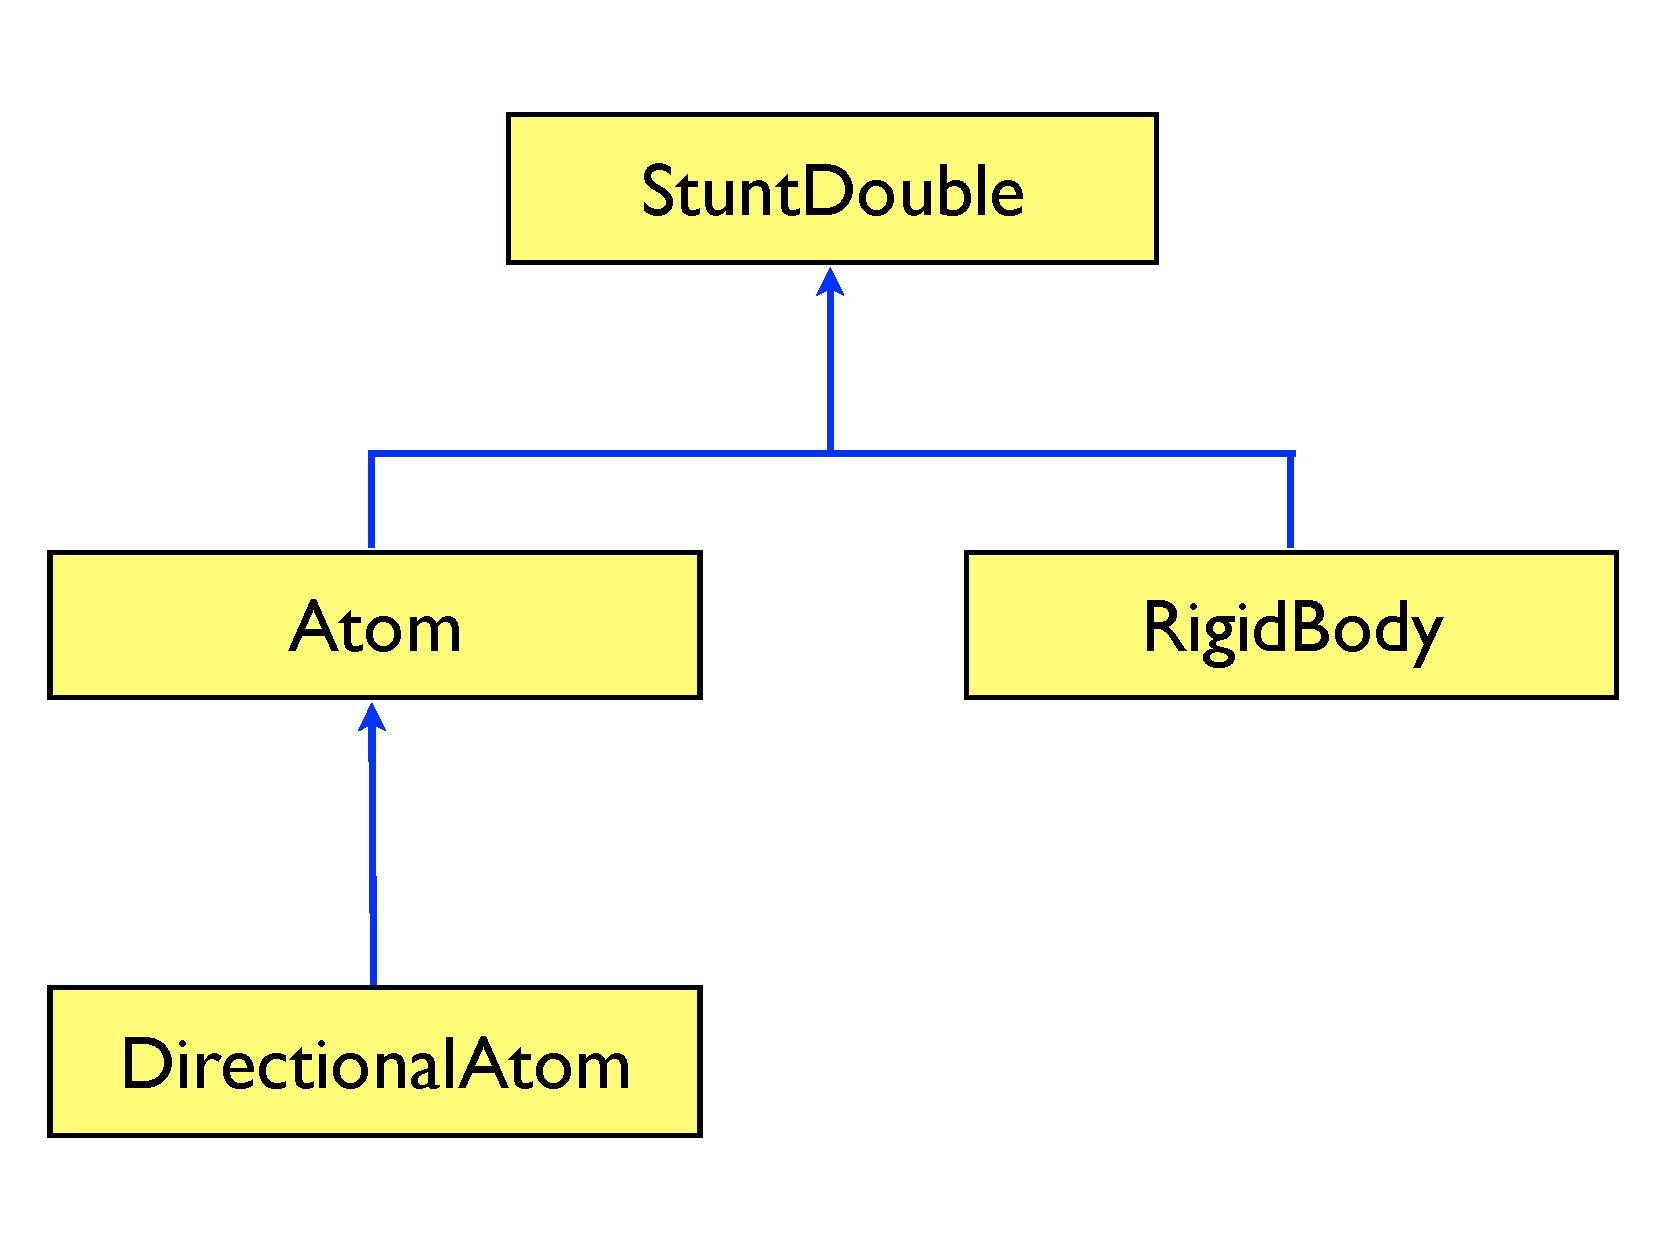
\includegraphics[width=3in]{heirarchy.pdf}
\caption[Class heirarchy for StuntDoubles in {\sc oopse}-4]{ \\ The
class heirarchy of StuntDoubles in {\sc oopse}-4. The selection
syntax allows the user to select any of the objects that are descended
from a StuntDouble.}
\label{oopseFig:heirarchy}
\end{figure}

\begin{itemize}
\item A {\bf StuntDouble} is {\it any} object that can be manipulated by the
integrators and minimizers. 
\item An {\bf Atom} is a fundamental point-particle that can be moved around during a simulation.
\item A {\bf DirectionalAtom} is an atom which has {\it orientational} as well as translational degrees of freedom.
\item A {\bf RigidBody} is a collection of {\bf Atom}s or {\bf
DirectionalAtom}s which behaves as a single unit.
\end{itemize} 

Every Molecule, Atom and DirectionalAtom in {\sc oopse} have their own names
which are specified in the {\tt .md} file. In contrast, RigidBodies are
denoted by their membership and index inside a particular molecule:
[MoleculeName]\_RB\_[index] (the contents inside the brackets
depend on the specifics of the simulation). The names of rigid bodies are
generated automatically. For example, the name of the first rigid body
in a DMPC molecule is DMPC\_RB\_0.

\section{\label{oopseSec:syntax}Syntax of the Select Command}

The most general form of the select command is: {\tt select {\it expression}}

This expression represents an arbitrary set of StuntDoubles (Atoms or
RigidBodies) in {\sc oopse}. Expressions are composed of either name
expressions, index expressions, predefined sets, user-defined
expressions, comparison operators, within expressions, or logical
combinations of the above expression types. Expressions can be
combined using parentheses and the Boolean operators.

\subsection{\label{oopseSec:logical}Logical expressions}

The logical operators allow complex queries to be constructed out of
simpler ones using the standard boolean connectives {\bf and}, {\bf
or}, {\bf not}. Parentheses can be used to alter the precedence of the
operators.

\begin{center}
\begin{tabular}{|ll|}
\hline
{\bf logical operator} & {\bf equivalent operator}  \\  
\hline
and & ``\&'', ``\&\&'' \\
or & ``$|$'', ``$||$'', ``,'' \\
not & ``!''  \\
\hline
\end{tabular}
\end{center}

\subsection{\label{oopseSec:name}Name expressions}

\begin{center}
\begin{tabular}{|llp{3in}|}
\hline
{\bf type of expression} & {\bf examples} & {\bf translation of
examples} \\
\hline
expression without ``.'' & select DMPC & select all StuntDoubles
belonging to all DMPC molecules \\
 & select C* & select all atoms which have atom types beginning with C
\\
 & select DMPC\_RB\_* & select all RigidBodies in DMPC molecules (but
only select the rigid bodies, and not the atoms belonging to them). \\
\hline
expression has one ``.'' & select TIP3P.O\_TIP3P & select the O\_TIP3P
atoms belonging to TIP3P molecules \\
 & select DMPC\_RB\_O.PO4 & select the PO4 atoms belonging to
the first 
RigidBody in each DMPC molecule \\
 & select DMPC.20 & select the twentieth StuntDouble in each DMPC
molecule \\
\hline
expression has two ``.''s & select DMPC.DMPC\_RB\_?.* &
select all atoms 
belonging to all rigid bodies within all DMPC molecules \\
\hline
\end{tabular}
\end{center}

\subsection{\label{oopseSec:index}Index expressions}

\begin{center}
\begin{tabular}{|lp{4in}|}
\hline
{\bf examples} & {\bf translation of examples} \\
\hline
select 20 & select all of the StuntDoubles belonging to Molecule 20 \\
select 20 to 30 & select all of the StuntDoubles belonging to
molecules which have global indices between 20 (inclusive) and 30
(exclusive) \\
\hline
\end{tabular}
\end{center}

\subsection{\label{oopseSec:predefined}Predefined sets}

\begin{center}
\begin{tabular}{|ll|}
\hline
{\bf keyword} & {\bf description} \\
\hline
all & select all StuntDoubles \\
none & select none of the StuntDoubles \\
\hline
\end{tabular}
\end{center}

\subsection{\label{oopseSec:userdefined}User-defined expressions}

Users can define arbitrary terms to represent groups of StuntDoubles,
and then use the define terms in select commands. The general form for
the define command is: {\bf define {\it term expression}}

Once defined, the user can specify such terms in boolean expressions

{\tt define SSDWATER SSD or SSD1 or SSDRF}

{\tt select SSDWATER}

\subsection{\label{oopseSec:comparison}Comparison expressions}

StuntDoubles can be selected by using comparision operators on their
properties. The general form for the comparison command is: a property
name, followed by a comparision operator and then a number. 

\begin{center}
\begin{tabular}{|l|l|}
\hline
{\bf property} & mass, charge \\
{\bf comparison operator} & ``$>$'', ``$<$'', ``$=$'', ``$>=$'',
``$<=$'', ``$!=$'' \\
\hline
\end{tabular}
\end{center}

For example, the phrase {\tt select mass > 16.0 and charge < -2}
wouldselect StuntDoubles which have mass greater than 16.0 and charges
less than -2.
 
\subsection{\label{oopseSec:within}Within expressions}

The ``within'' keyword allows the user to select all StuntDoubles
within the specified distance (in Angstroms) from a selection,
including the selected atom itself. The general form for within
selection is: {\tt select within(distance, expression)}
 
For example, the phrase {\tt select within(2.5, PO4 or NC4)} would
select all StuntDoubles which are within 2.5 angstroms of PO4 or NC4
atoms.

\section{\label{oopseSec:tools}Tools which use the selection command}

\subsection{\label{oopseSec:Dump2XYZ}Dump2XYZ}

Dump2XYZ can transform an OOPSE dump file into a xyz file which can
be opened by other molecular dynamics viewers such as Jmol and
VMD. The options available for Dump2XYZ are as follows:


\begin{longtable}[c]{|EFG|}
\caption{Dump2XYZ Command-line Options}
\\ \hline
{\bf option} & {\bf verbose option} & {\bf behavior} \\ \hline
\endhead
\hline
\endfoot
  -h & {\tt -{}-help} &                        Print help and exit \\
  -V & {\tt -{}-version} &                     Print version and exit \\
  -i & {\tt -{}-input=filename}  &             input dump file \\
  -o & {\tt -{}-output=filename} &             output file name \\
  -n & {\tt -{}-frame=INT}   &                 print every n frame  (default=`1') \\
  -w & {\tt -{}-water}       &                 skip the the waters  (default=off) \\
  -m & {\tt -{}-periodicBox} &                 map to the periodic box  (default=off)\\
  -z & {\tt -{}-zconstraint}  &                replace the atom types of zconstraint molecules  (default=off) \\
  -r & {\tt -{}-rigidbody}  &                  add a pseudo COM atom to rigidbody  (default=off) \\
  -t & {\tt -{}-watertype} &                   replace the atom type of water model (default=on) \\
  -b & {\tt -{}-basetype}  &                   using base atom type  (default=off) \\
     & {\tt -{}-repeatX=INT}  &                 The number of images to repeat in the x direction  (default=`0') \\
     & {\tt -{}-repeatY=INT} &                 The number of images to repeat in the y direction  (default=`0') \\
     &  {\tt -{}-repeatZ=INT}  &                The number of images to repeat in the z direction  (default=`0') \\
  -s & {\tt -{}-selection=selection script} & By specifying {\tt -{}-selection}=``selection command'' with Dump2XYZ, the user can select an arbitrary set of StuntDoubles to be
converted. \\ 
     & {\tt -{}-originsele} & By specifying {\tt -{}-originsele}=``selection command'' with Dump2XYZ, the user can re-center the origin of the system around a specific StuntDouble \\ 
     & {\tt -{}-refsele} &  In order to rotate the system, {\tt -{}-originsele} and {\tt -{}-refsele} must be given to define the new coordinate set. A StuntDouble which contains a dipole (the direction of the dipole is always (0, 0, 1) in body frame) is specified by {\tt -{}-originsele}. The new x-z plane is defined by the direction of the dipole and the StuntDouble is specified by {\tt -{}-refsele}.
\end{longtable}


\subsection{\label{oopseSec:StaticProps}StaticProps}

{\tt StaticProps} can compute properties which are averaged over some
or all of the configurations that are contained within a dump file.
The most common example of a static property that can be computed is
the pair distribution function between atoms of type $A$ and other
atoms of type $B$, $g_{AB}(r)$.  StaticProps can also be used to
compute the density distributions of other molecules in a reference
frame {\it fixed to the body-fixed reference frame} of a selected atom
or rigid body.

There are five seperate radial distribution functions availiable in
OOPSE. Since every radial distrbution function invlove the calculation
between pairs of bodies, {\tt -{}-sele1} and {\tt -{}-sele2} must be specified to tell
StaticProps which bodies to include in the calculation.

\begin{description}
\item[{\tt -{}-gofr}] Computes the pair distribution function,
\begin{equation*}
g_{AB}(r) = \frac{1}{\rho_B}\frac{1}{N_A} \langle \sum_{i \in A}
\sum_{j \in B} \delta(r - r_{ij}) \rangle
\end{equation*}
\item[{\tt -{}-r\_theta}] Computes the angle-dependent pair distribution
function. The angle is defined by the intermolecular vector $\vec{r}$ and
$z$-axis of DirectionalAtom A,
\begin{equation*}
g_{AB}(r, \cos \theta) = \frac{1}{\rho_B}\frac{1}{N_A} \langle \sum_{i \in A}
\sum_{j \in B} \delta(r - r_{ij}) \delta(\cos \theta_{ij} - \cos \theta)\rangle
\end{equation*}
\item[{\tt -{}-r\_omega}] Computes the angle-dependent pair distribution
function. The angle is defined by the $z$-axes of the two
DirectionalAtoms A and B. 
\begin{equation*}
g_{AB}(r, \cos \omega) = \frac{1}{\rho_B}\frac{1}{N_A} \langle \sum_{i \in A}
\sum_{j \in B} \delta(r - r_{ij}) \delta(\cos \omega_{ij} - \cos \omega)\rangle
\end{equation*}
\item[{\tt -{}-theta\_omega}] Computes the pair distribution in the angular
space $\theta, \omega$ defined by the two angles mentioned above.
\begin{equation*}
g_{AB}(\cos\theta, \cos \omega) = \frac{1}{\rho_B}\frac{1}{N_A} \langle \sum_{i \in A}
\sum_{j \in B} \langle \delta(\cos \theta_{ij} - \cos \theta)
\delta(\cos \omega_{ij} - \cos \omega)\rangle
\end{equation*}
\item[{\tt -{}-gxyz}] Calculates the density distribution of particles of type
B in the body frame of particle A. Therefore, {\tt -{}-originsele} and
{\tt -{}-refsele} must be given to define A's internal coordinate set as
the reference frame for the calculation.
\end{description}

The vectors (and angles) associated with these angular pair
distribution functions are most easily seen in the figure below:

\begin{figure}
\centering
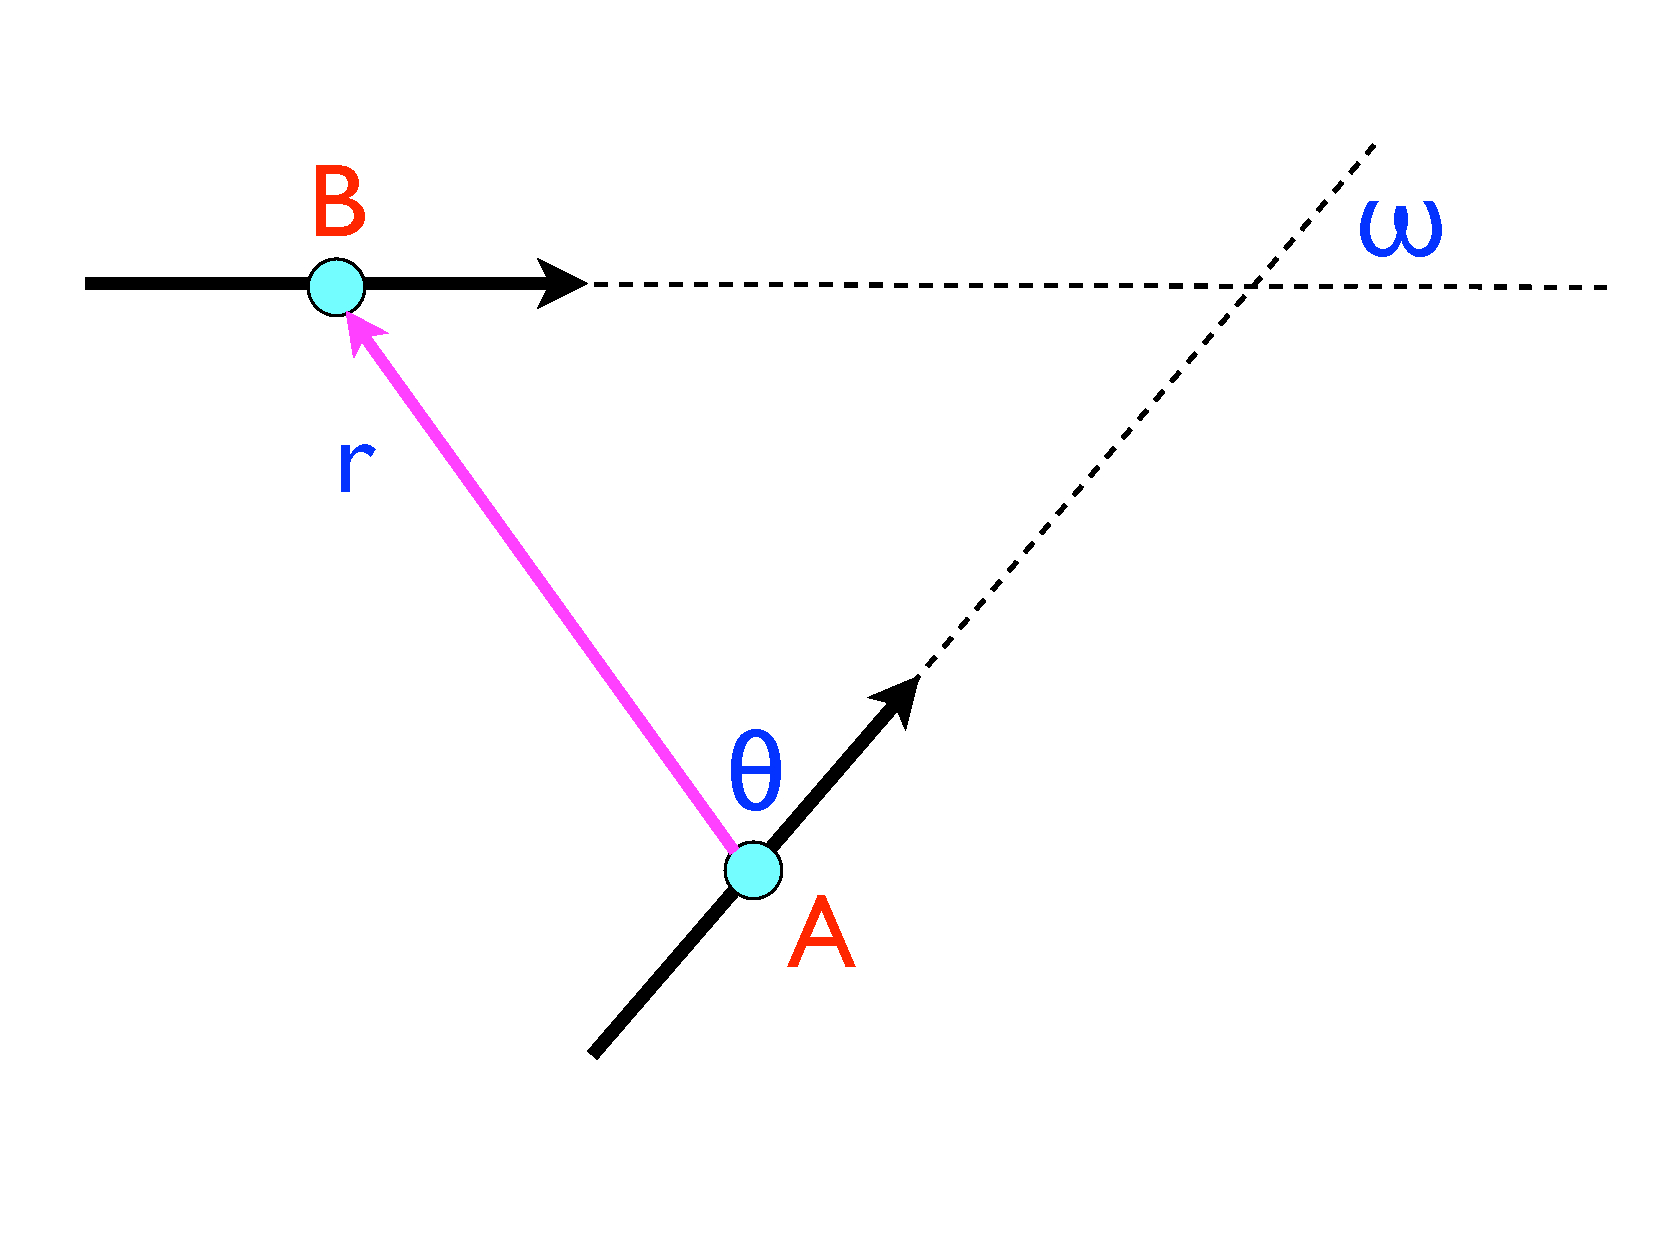
\includegraphics[width=3in]{definition.pdf}
\caption[Definitions of the angles between directional objects]{ \\ Any
two directional objects (DirectionalAtoms and RigidBodies) have a set
of two angles ($\theta$, and $\omega$) between the z-axes of their
body-fixed frames.} 
\label{oopseFig:gofr}
\end{figure}

The options available for {\tt StaticProps} are as follows:
\begin{longtable}[c]{|EFG|}
\caption{StaticProps Command-line Options}
\\ \hline
{\bf option} & {\bf verbose option} & {\bf behavior} \\ \hline
\endhead
\hline
\endfoot
  -h& {\tt -{}-help}                    &  Print help and exit \\
  -V& {\tt -{}-version}                 &  Print version and exit \\
  -i& {\tt -{}-input=filename}          &  input dump file \\
  -o& {\tt -{}-output=filename}         &  output file name \\
  -n& {\tt -{}-step=INT}                &  process every n frame  (default=`1') \\
  -r& {\tt -{}-nrbins=INT}              &  number of bins for distance  (default=`100') \\
  -a& {\tt -{}-nanglebins=INT}          &  number of bins for cos(angle)  (default= `50') \\
  -l& {\tt -{}-length=DOUBLE}           &  maximum length (Defaults to 1/2 smallest length of first frame) \\
    & {\tt -{}-sele1=selection script}   & select the first StuntDouble set \\
    & {\tt -{}-sele2=selection script}   & select the second StuntDouble set \\
    & {\tt -{}-sele3=selection script}   & select the third StuntDouble set \\
    & {\tt -{}-refsele=selection script} & select reference (can only be used with {\tt -{}-gxyz}) \\
    & {\tt -{}-molname=STRING}           & molecule name \\
    & {\tt -{}-begin=INT}                & begin internal index \\
    & {\tt -{}-end=INT}                  & end internal index \\
\hline
\multicolumn{3}{|l|}{One option from the following group of options is required:} \\
\hline
    &  {\tt -{}-gofr}                    &  $g(r)$ \\
    &  {\tt -{}-r\_theta}                 &  $g(r, \cos(\theta))$ \\
    &  {\tt -{}-r\_omega}                 &  $g(r, \cos(\omega))$ \\
    &  {\tt -{}-theta\_omega}             &  $g(\cos(\theta), \cos(\omega))$ \\
    &  {\tt -{}-gxyz}                    &  $g(x, y, z)$ \\
    &  {\tt -{}-p2}                      &  $P_2$ order parameter ({\tt -{}-sele1} and {\tt -{}-sele2} must be specified) \\
    &  {\tt -{}-scd}                     &  $S_{CD}$ order parameter(either {\tt -{}-sele1}, {\tt -{}-sele2}, {\tt -{}-sele3} are specified or {\tt -{}-molname}, {\tt -{}-begin}, {\tt -{}-end} are specified) \\
    &  {\tt -{}-density}                 &  density plot ({\tt -{}-sele1} must be specified) \\
    &  {\tt -{}-slab\_density}           &  slab density ({\tt -{}-sele1} must be specified)
\end{longtable}

\subsection{\label{oopseSec:DynamicProps}DynamicProps}

{\tt DynamicProps} computes time correlation functions from the
configurations stored in a dump file.  Typical examples of time
correlation functions are the mean square displacement and the
velocity autocorrelation functions.   Once again, the selection syntax
can be used to specify the StuntDoubles that will be used for the
calculation.  A general time correlation function can be thought of
as:
\begin{equation}
C_{AB}(t) = \langle \vec{u}_A(t) \cdot \vec{v}_B(0) \rangle
\end{equation}
where $\vec{u}_A(t)$ is a vector property associated with an atom of
type $A$ at time $t$, and $\vec{v}_B(t^{\prime})$ is a different vector
property associated with an atom of type $B$ at a different time
$t^{\prime}$.  In most autocorrelation functions, the vector properties
($\vec{v}$ and $\vec{u}$) and the types of atoms ($A$ and $B$) are
identical, and the three calculations built in to {\tt DynamicProps}
make these assumptions.  It is possible, however, to make simple
modifications to the {\tt DynamicProps} code to allow the use of {\it
cross} time correlation functions (i.e. with different vectors).  The
ability to use two selection scripts to select different types of
atoms is already present in the code.

The options available for DynamicProps are as follows:
\begin{longtable}[c]{|EFG|}
\caption{DynamicProps Command-line Options}
\\ \hline
{\bf option} & {\bf verbose option} & {\bf behavior} \\ \hline
\endhead
\hline
\endfoot
  -h& {\tt -{}-help}                   & Print help and exit \\
  -V& {\tt -{}-version}                & Print version and exit \\
  -i& {\tt -{}-input=filename}         & input dump file \\
  -o& {\tt -{}-output=filename}        & output file name \\
    & {\tt -{}-sele1=selection script} & select first StuntDouble set \\
    & {\tt -{}-sele2=selection script} & select second StuntDouble set (if sele2 is not set, use script from sele1) \\
\hline
\multicolumn{3}{|l|}{One option from the following group of options is required:} \\
\hline
  -r& {\tt -{}-rcorr}                  & compute mean square displacement \\
  -v& {\tt -{}-vcorr}                  & compute velocity correlation function \\
  -d& {\tt -{}-dcorr}                  & compute dipole correlation function
\end{longtable}

\chapter{\label{oopseSec:PreparingInput} Preparing Input Configurations}

{\sc oopse} version 4 comes with a few utility programs to aid in
setting up initial configuration and meta-data files.  Usually, a user
is interested in either importing a structure from some other format
(usually XYZ or PDB), or in building an initial configuration in some
perfect crystalline lattice.  The programs bundled with {\sc oopse}
which import coordinate files are {\tt atom2md}, {\tt xyz2md}, and
{\tt pdb2md}. The programs which generate perfect crystals are called
{\tt SimpleBuilder} and {\tt RandomBuilder}

\section{\label{oopseSec:atom2md}atom2md, xyz2md, and pdb2md}

{\tt atom2md}, {\tt xyz2md}, and {\tt pdb2md} attempt to construct
{\tt .md} files from a single file containing only atomic coordinate
information.  To do this task, they make reasonable guesses about
bonding from the distance between atoms in the coordinate, and attempt
to identify other terms in the potential energy from the topology of
the graph of discovered bonds.  This procedure is not perfect, and the
user should check the discovered bonding topology that is contained in
the {\tt $<$MetaData$>$} block in the file that is generated.

Typically, the user would run:

{\tt atom2md $<$input spec$>$ [Options]}

Here {\tt $<$input spec$>$} can be used to specify the type of file being
used for configuration input. I.e. using {\tt -ipdb} specifies that the
input file contains coordinate information in the PDB format.

The options available for atom2md are as follows:
\begin{longtable}[c]{|HI|}
\caption{atom2md Command-line Options}
\\ \hline
{\bf option} &  {\bf behavior} \\ \hline
\endhead
\hline
\endfoot
  -f \# & Start import at molecule \# specified \\
  -l \# & End import at molecule \# specified \\
  -t  & All input files describe a single molecule \\
  -e & Continue with next object after error, if possible \\
  -z & Compress the output with gzip \\
  -H & Outputs this help text \\
  -Hxxx & (xxx is file format ID e.g. -Hpdb) gives format info \\
  -Hall & Outputs details of all formats \\
  -V & Outputs version number \\
\hline
\multicolumn{2}{|l|}{The following file formats are recognized:}\\
\hline
  ent & Protein Data Bank format \\
  in & {\sc oopse} cartesian coordinates format \\
  pdb & Protein Data Bank format \\
  prep & Amber Prep format  \\
  xyz & XYZ cartesian coordinates format \\
\hline
\multicolumn{2}{|l|}{More specific info and options are available
using -H$<$format-type$>$, e.g. -Hpdb} 
\end{longtable}

The specific programs {\tt xyz2md} and {\tt pdb2md} are identical
to {\tt atom2md}, but they use a specific input format and do not
expect the the input specifier on the command line. 

\section{\label{oopseSec:SimpleBuilder}SimpleBuilder}

{\tt SimpleBuilder} creates simple lattice structures.  It requires an
initial, but skeletal OOPSE file to specify the components that are to
be placed on the lattice.  The total number of placed molecules will
be shown at the top of the configuration file that is generated, and
that number may not match the original meta-data file, so a new
meta-data file is also generated which matches the lattice structure.

The options available for SimpleBuilder are as follows:
\begin{longtable}[c]{|EFG|}
\caption{SimpleBuilder Command-line Options}
\\ \hline
{\bf option} & {\bf verbose option} & {\bf behavior} \\ \hline
\endhead
\hline
\endfoot
  -h& {\tt -{}-help}               & Print help and exit\\
  -V& {\tt -{}-version}            & Print version and exit\\
  -o& {\tt -{}-output=STRING}      & Output file name\\
   &  {\tt -{}-density=DOUBLE}     & density ($\mathrm{g~cm}^{-3}$)\\
    &  {\tt -{}-nx=INT}            &  number of unit cells in x\\
    &  {\tt -{}-ny=INT}           &  number of unit cells in y\\
    &  {\tt -{}-nz=INT}            &  number of unit cells in z
\end{longtable}

\section{\label{oopseSec:Hydro}Hydro}
{\tt Hydro} generates {\tt .diff} file which is required when a Langevin
Dynamics simulation using approximate models (supports Bead Model and
Rough Shell Model) is performed. To generate the {\tt }.diff file, the
meta-data file is needed as the input file. The viscosity of the fluid
flow (solvent) and the temperature of the system have to be defined in
meta-data file. If the approximate model is {\tt Rough Shell Model},
the {\tt beadSize} which is the diameter of every beads must be
specified in meta-data file.

The options available for Hydro are as follows:
\begin{longtable}[c]{|EFG|}
\caption{Hydro Command-line Options}
\\ \hline
{\bf option} & {\bf verbose option} & {\bf behavior} \\ \hline
\endhead
\hline
\endfoot
  -h& {\tt -{}-help}               & Print help and exit\\
  -V& {\tt -{}-version}            & Print version and exit\\
  -i& {\tt -{}-input=filename}     & input MetaData (md) file\\
  -o& {\tt -{}-output=STRING}      & Output file name\\
   &  {\tt -{}-model=STRING}     & hydrodynamics model (supports
RoughShell and BeadModel)\\
  -b&  {\tt -{}-beads}            & generate the beads only,
hydrodynamics will be performed (default=off)\\
\end{longtable}


\chapter{\label{oopseSec:parallelization} Parallel Simulation Implementation}

Although processor power is continually improving, it is still
unreasonable to simulate systems of more than 10,000 atoms on a single
processor. To facilitate study of larger system sizes or smaller
systems for longer time scales, parallel methods were developed to
allow multiple CPU's to share the simulation workload. Three general
categories of parallel decomposition methods have been developed:
these are the atomic,\cite{Fox88} spatial~\cite{plimpton95} and
force~\cite{Paradyn} decomposition methods.

Algorithmically simplest of the three methods is atomic decomposition,
where $N$ particles in a simulation are split among $P$ processors for
the duration of the simulation. Computational cost scales as an
optimal $\mathcal{O}(N/P)$ for atomic decomposition. Unfortunately, all
processors must communicate positions and forces with all other
processors at every force evaluation, leading the communication costs
to scale as an unfavorable $\mathcal{O}(N)$, \emph{independent of the
number of processors}. This communication bottleneck led to the
development of spatial and force decomposition methods, in which
communication among processors scales much more favorably. Spatial or
domain decomposition divides the physical spatial domain into 3D boxes
in which each processor is responsible for calculation of forces and
positions of particles located in its box. Particles are reassigned to
different processors as they move through simulation space. To
calculate forces on a given particle, a processor must simply know the
positions of particles within some cutoff radius located on nearby
processors rather than the positions of particles on all
processors. Both communication between processors and computation
scale as $\mathcal{O}(N/P)$ in the spatial method. However, spatial
decomposition adds algorithmic complexity to the simulation code and
is not very efficient for small $N$, since the overall communication
scales as the surface to volume ratio $\mathcal{O}(N/P)^{2/3}$ in
three dimensions.

The parallelization method used in {\sc oopse} is the force
decomposition method.\cite{hendrickson:95} Force decomposition assigns
particles to processors based on a block decomposition of the force
matrix. Processors are split into an optimally square grid forming row
and column processor groups. Forces are calculated on particles in a
given row by particles located in that processor's column
assignment. One deviation from the algorithm described by Hendrickson
{\it et al.} is the use of column ordering based on the row indexes
preventing the need for a transpose operation necessitating a second
communication step when gathering the final force components.  Force
decomposition is less complex to implement than the spatial method but
still scales computationally as $\mathcal{O}(N/P)$ and scales as
$\mathcal{O}(N/\sqrt{P})$ in communication cost. Plimpton has also
found that force decompositions scale more favorably than spatial
decompositions for systems up to 10,000 atoms and favorably compete
with spatial methods up to 100,000 atoms.\cite{plimpton95}
 
\chapter{\label{oopseSec:conclusion}Conclusion}

We have presented a new parallel simulation program called {\sc
oopse}. This program offers some novel capabilities, but mostly makes
available a library of modern object-oriented code for the scientific
community to use freely.  Notably, {\sc oopse} can handle symplectic
integration of objects (atoms and rigid bodies) which have
orientational degrees of freedom.  It can also work with transition
metal force fields and point-dipoles. It is capable of scaling across
multiple processors through the use of force based decomposition. It
also implements several advanced integrators allowing the end user
control over temperature and pressure. In addition, it is capable of
integrating constrained dynamics through both the {\sc rattle}
algorithm and the $z$-constraint method.

We encourage other researchers to download and apply this program to
their own research problems.  By making the code available, we hope to
encourage other researchers to contribute their own code and make it a
more powerful package for everyone in the molecular dynamics community
to use.  All source code for {\sc oopse} is available for download at
{\tt http://oopse.org}.

\chapter{Acknowledgments}

Development of {\sc oopse} was funded by a New Faculty Award from the
Camille and Henry Dreyfus Foundation and by the National Science
Foundation under grant CHE-0134881. Computation time was provided by
the Notre Dame Bunch-of-Boxes (B.o.B) computer cluster under NSF grant
DMR-0079647.


\bibliographystyle{jcc}
\bibliography{oopseDoc}

\end{document}
